\documentclass{article}

\usepackage{graphicx}

\usepackage[margin=0.5cm]{geometry}
\usepackage{amsmath}
\usepackage{indentfirst}
\usepackage{hyperref}
\usepackage{multirow}
\usepackage{comment}

\newcommand{\cosa}{\cos\hat\alpha}
\newcommand{\size}{0.33\textwidth}
\newcommand{\pt}{p_\text{T}}

\begin{document}

\title{Data vs MC comparison for 8 and 13 TeV $Z$}
\author{Mariana Ara\'ujo (LIP)}
\maketitle

\begin{comment}
\section{Procedure}

One MC distribution is obtained, under the following conditions:
\begin{itemize}
\item Generating $Z$ ($M=91.1876$ GeV) at $\sqrt{s}=8$ TeV.
\item CHANGE FROM THIS POINT ON TO BE Z GENERATION
\item $s^*$ generated by sampling $h(s^*)$, where
$$ h(s^*) = \left(s^*\right)^{-\beta}$$
\item Using CT14 NNLO gluon PDF with the aid of LHAPDF. $x_1$ (or $x_2$) generated uniformly in $\log(x)$ and a weight of $f(x_1)f(x_2)$ is considered for each event, where $f(x)$ is the PDF.
\item $\cos\hat\alpha$ generated uniformly and a weight of $g(s^*, \cos\hat\alpha)$ is considered, where
$$g(s^*, \cos\hat\alpha) = \left[\frac{1}{(E^*+p^*\cdot\cos\hat\alpha)^\rho}+\frac{1}{(E^*-p^*\cdot\cos\hat\alpha)^\rho}\right]\frac{(E^*)^\rho/2}{(1+\varepsilon-\cos\hat\alpha^2)^\delta},$$
\item We use the parameters $(\beta, \rho, \delta) = (2, 2, 0)$. Note that these are not obtained through any fit, but simply suggested values that seemed to agree well with data from previous tests.
\end{itemize}

We compare these samples with data by plotting histograms of the $\xi$ distributions in given bins of $y$, together with the ATLAS measurements of the $Z$ production cross section.

The comparison plots are presented in the next pages. 
\end{comment}
\clearpage

\newgeometry{margin = 0.5cm}

\begin{figure}[h!]
\centering
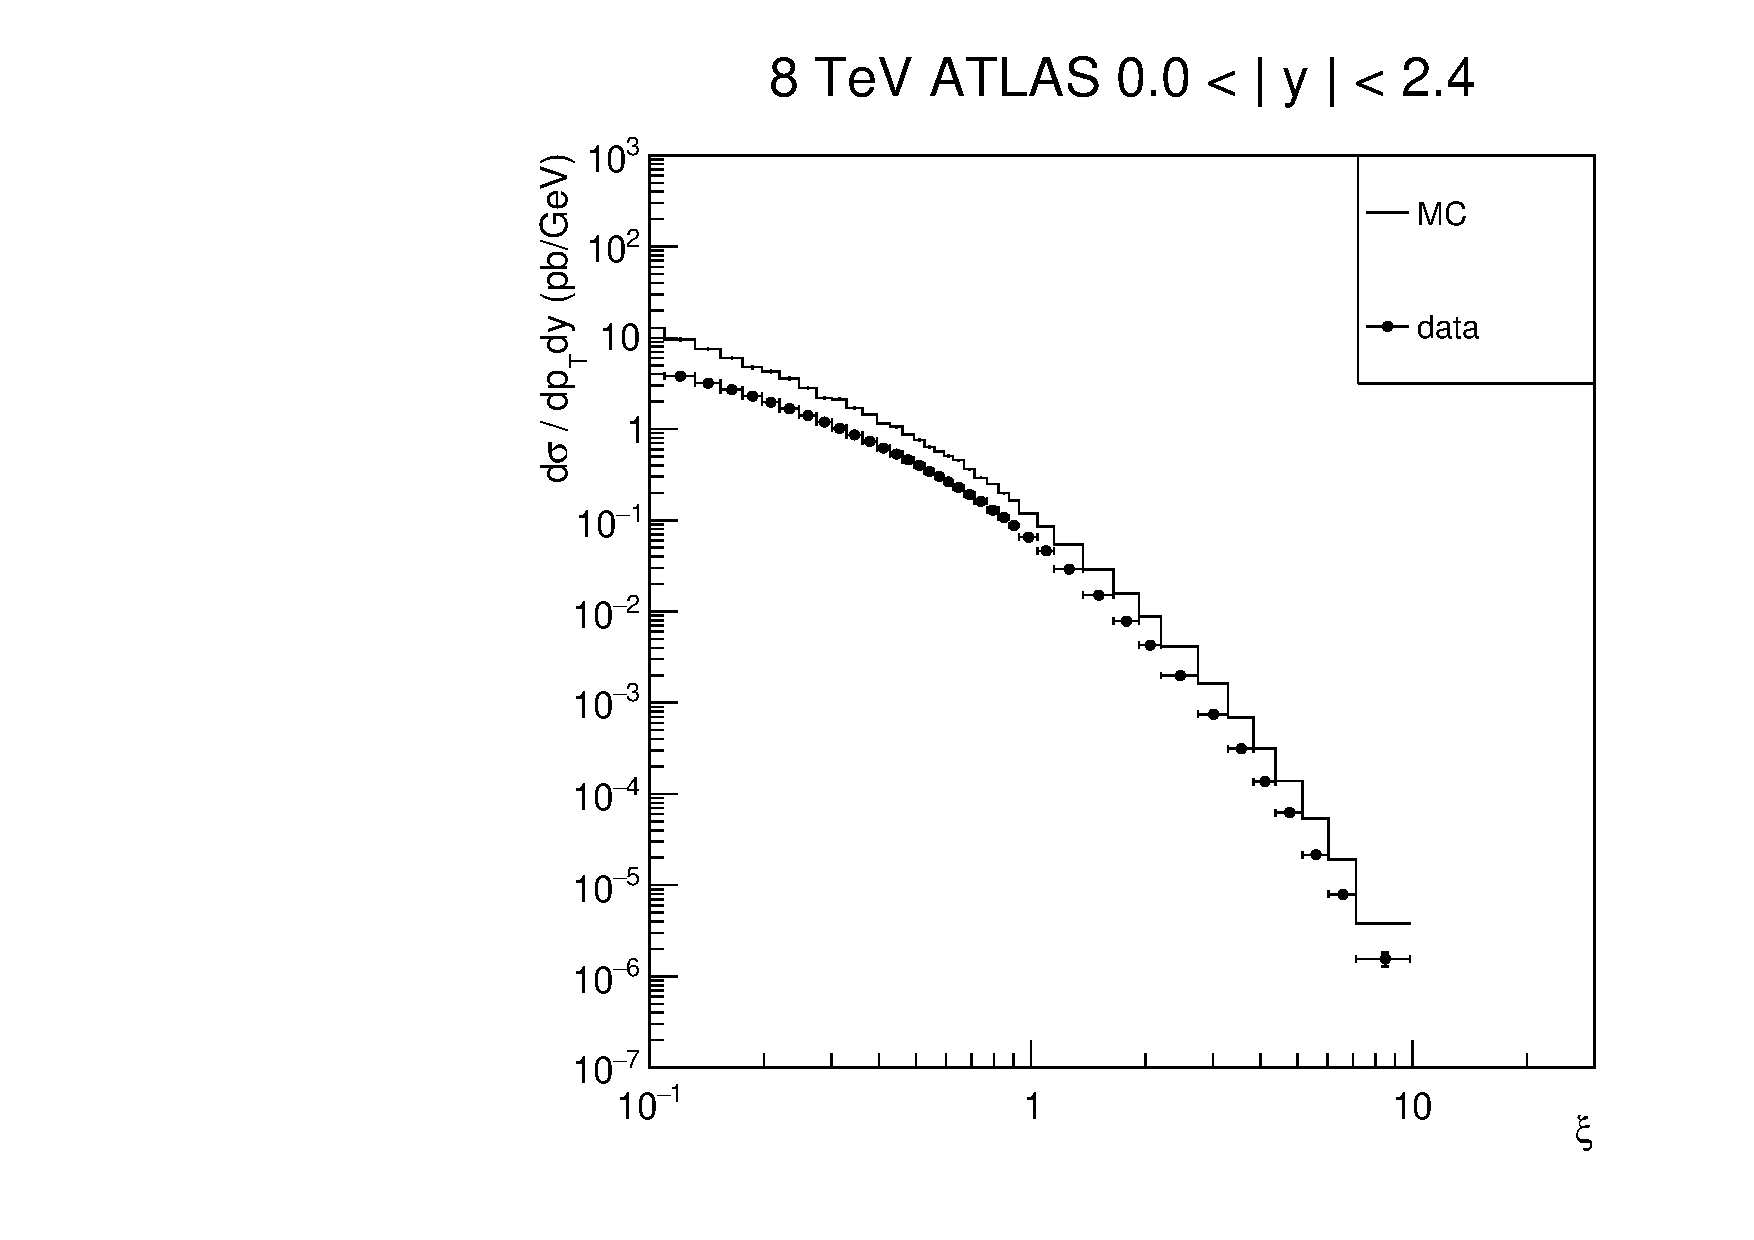
\includegraphics[width = 0.4\textwidth]{xi_8_A_y0.pdf}
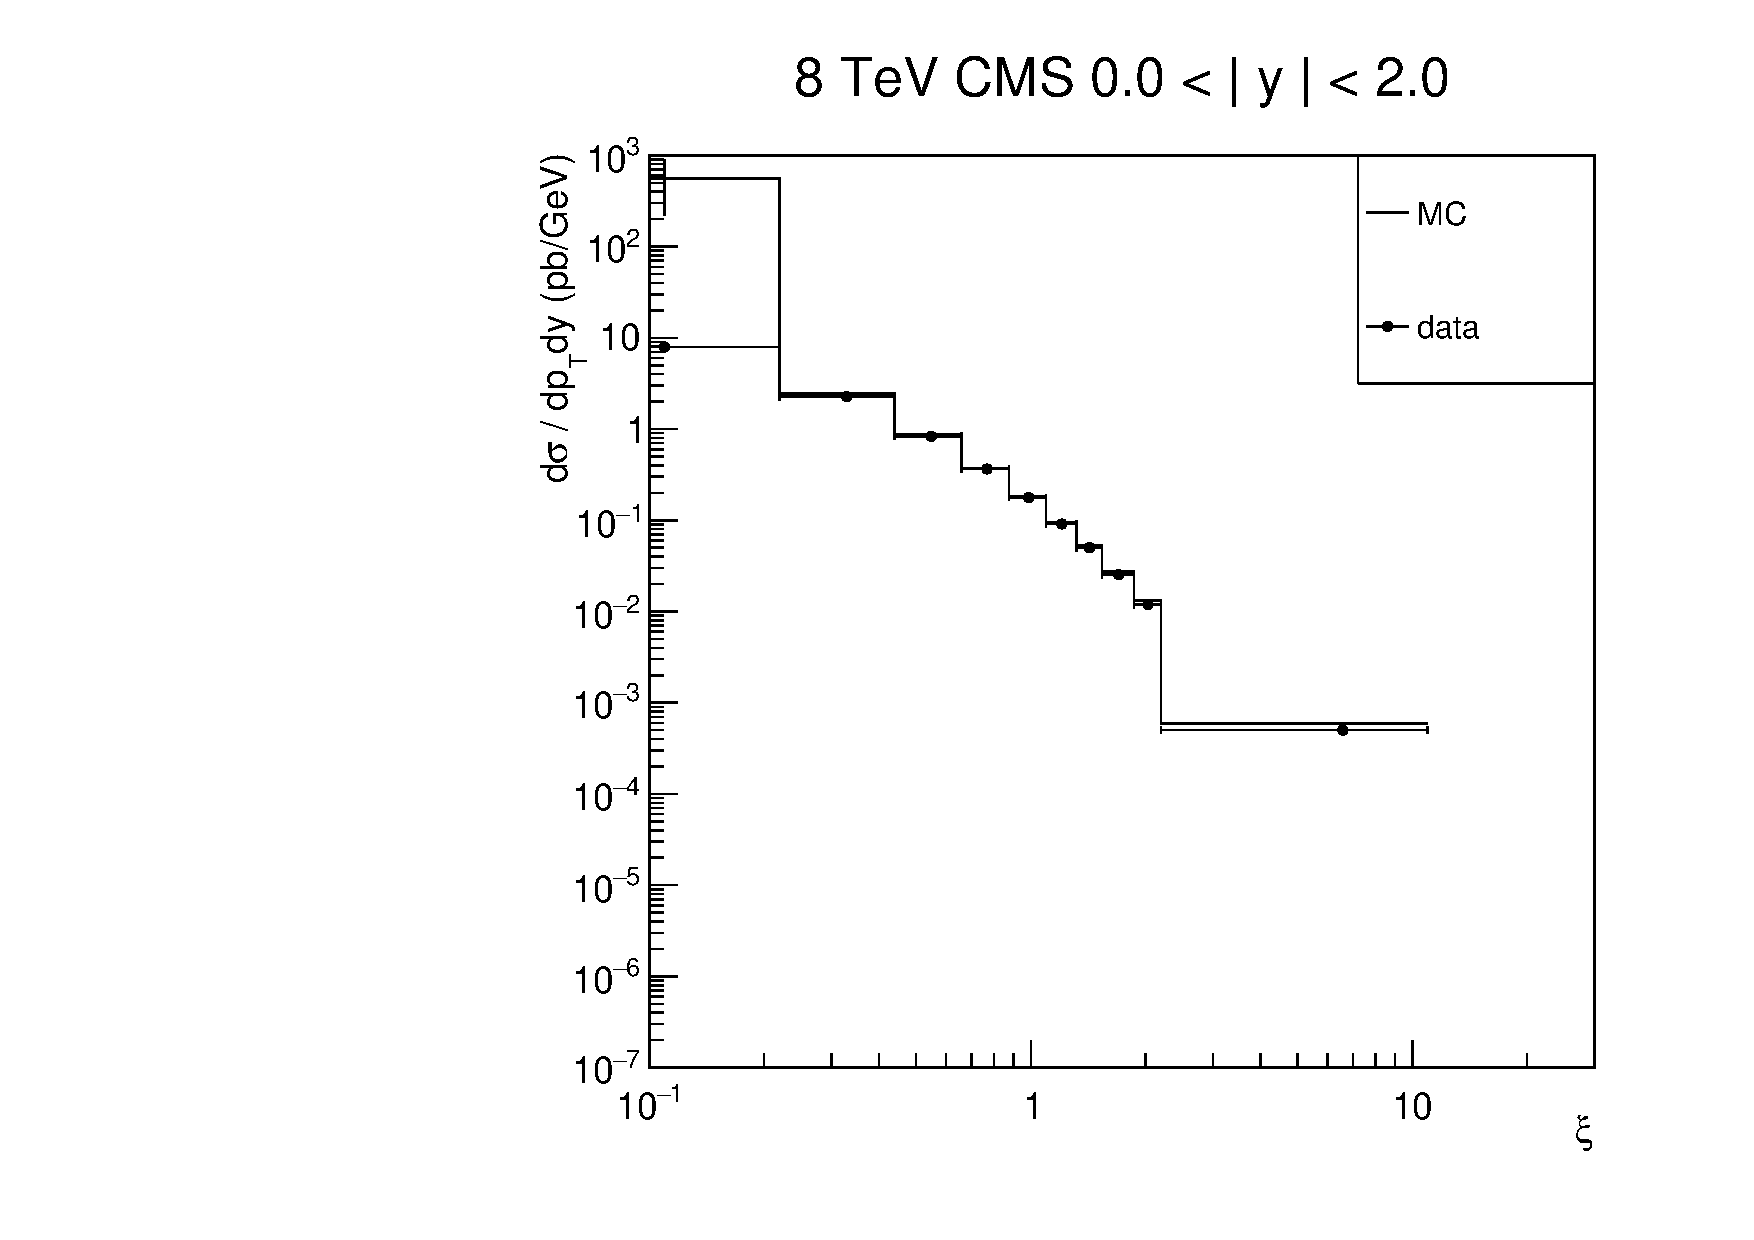
\includegraphics[width = 0.4\textwidth]{xi_8_C_y0.pdf}

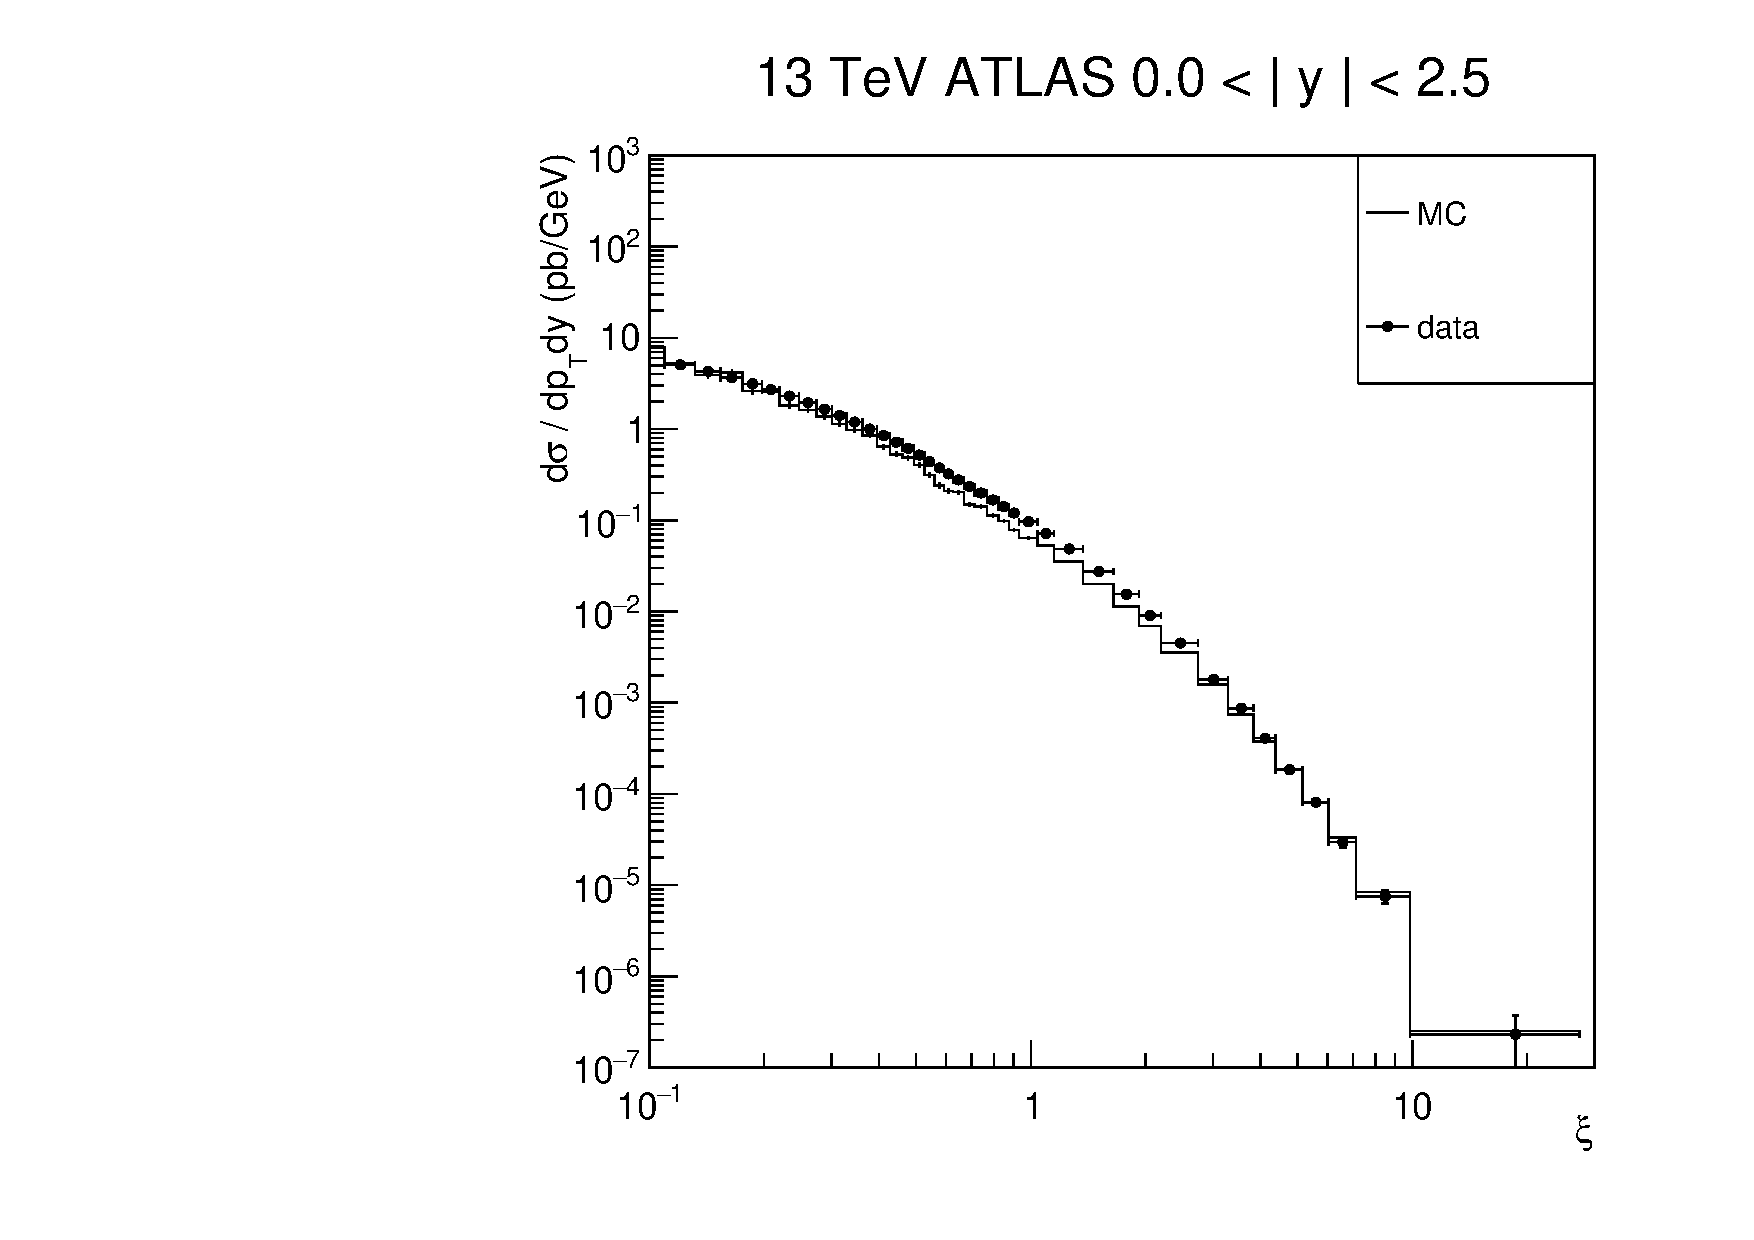
\includegraphics[width = 0.4\textwidth]{xi_13_A_y0.pdf}
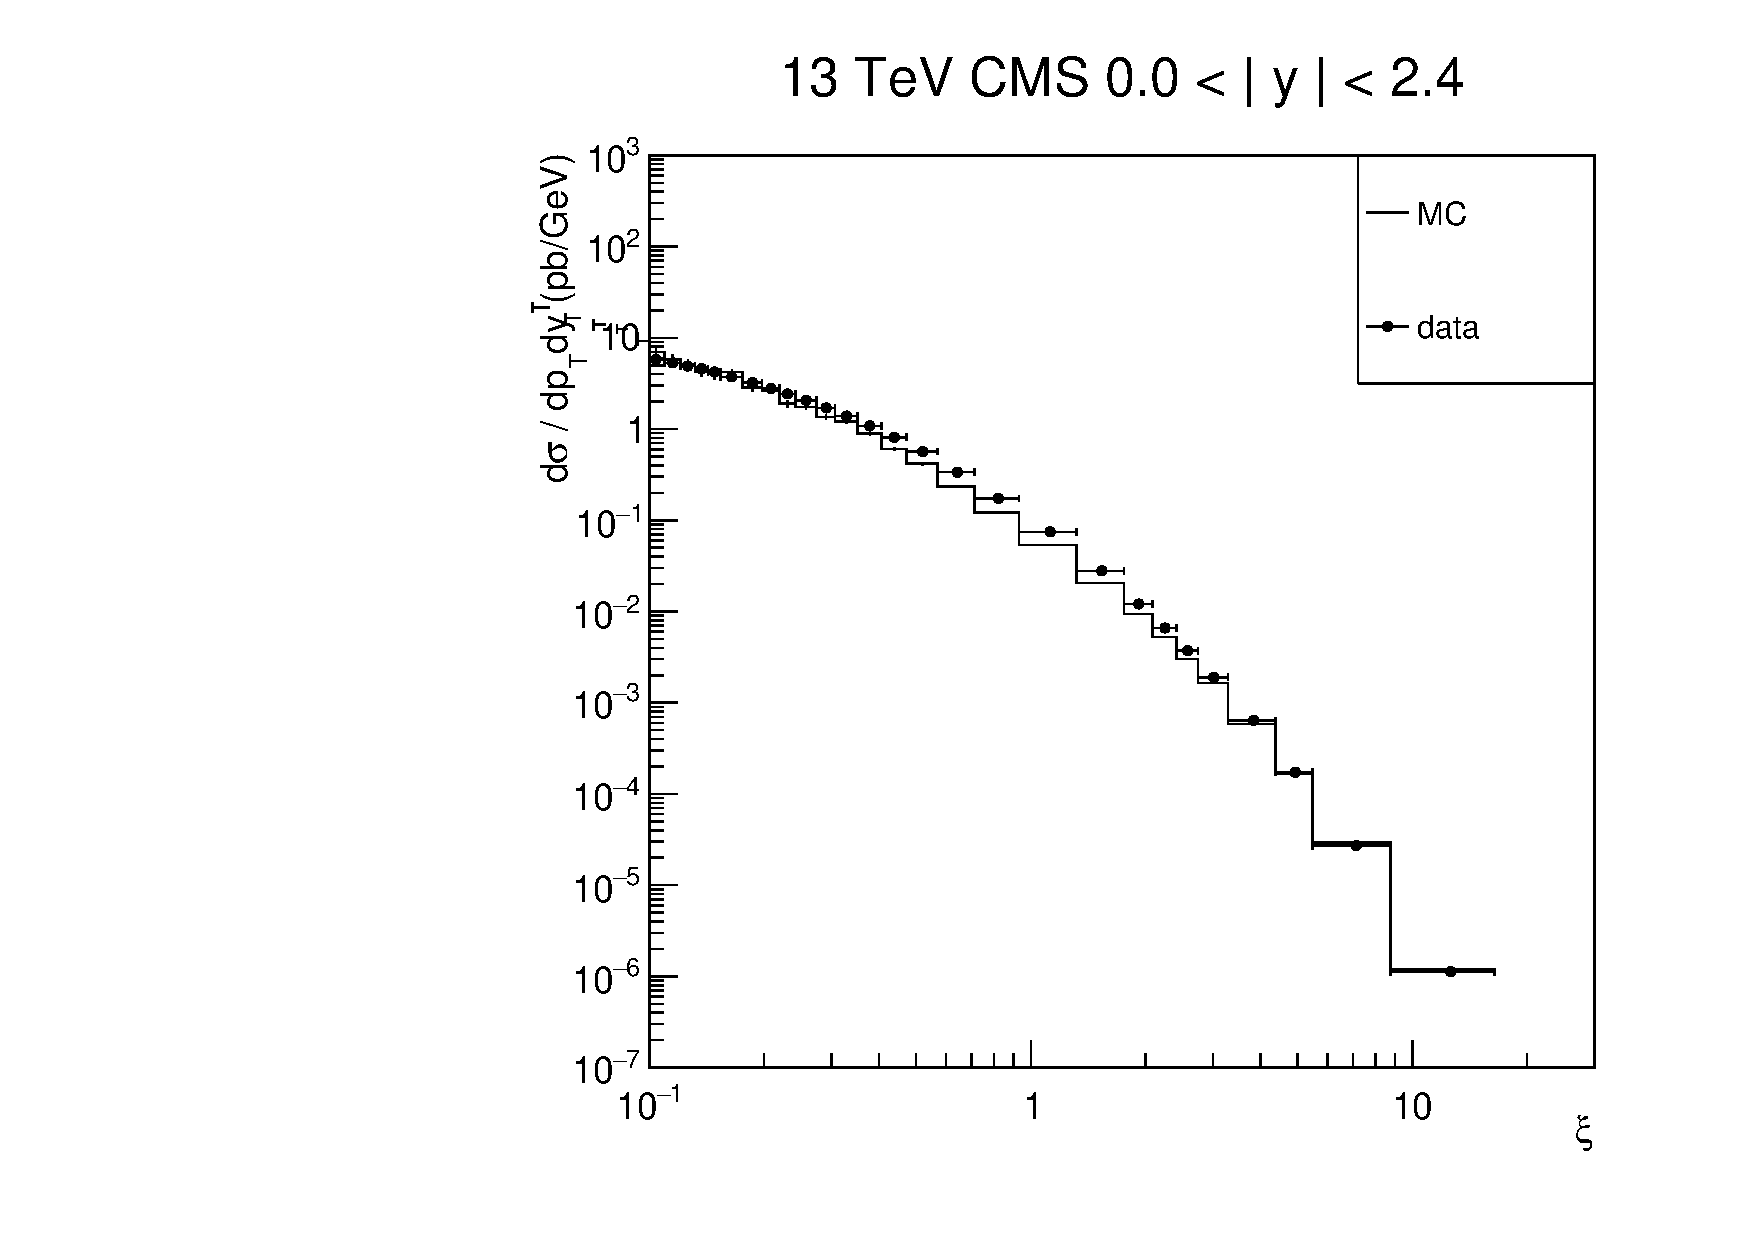
\includegraphics[width = 0.4\textwidth]{xi_13_C_y0.pdf}
%\caption{Comparison between MC $\xi$ distribution and data points in the six $y$ bins of the data, for 8 TeV. All histograms divided by total nr events and multiplied by same normalization factor. Data is not scaled.}\label{f:xi_comp}
\end{figure}

\clearpage

\begin{figure}[h!]
\centering
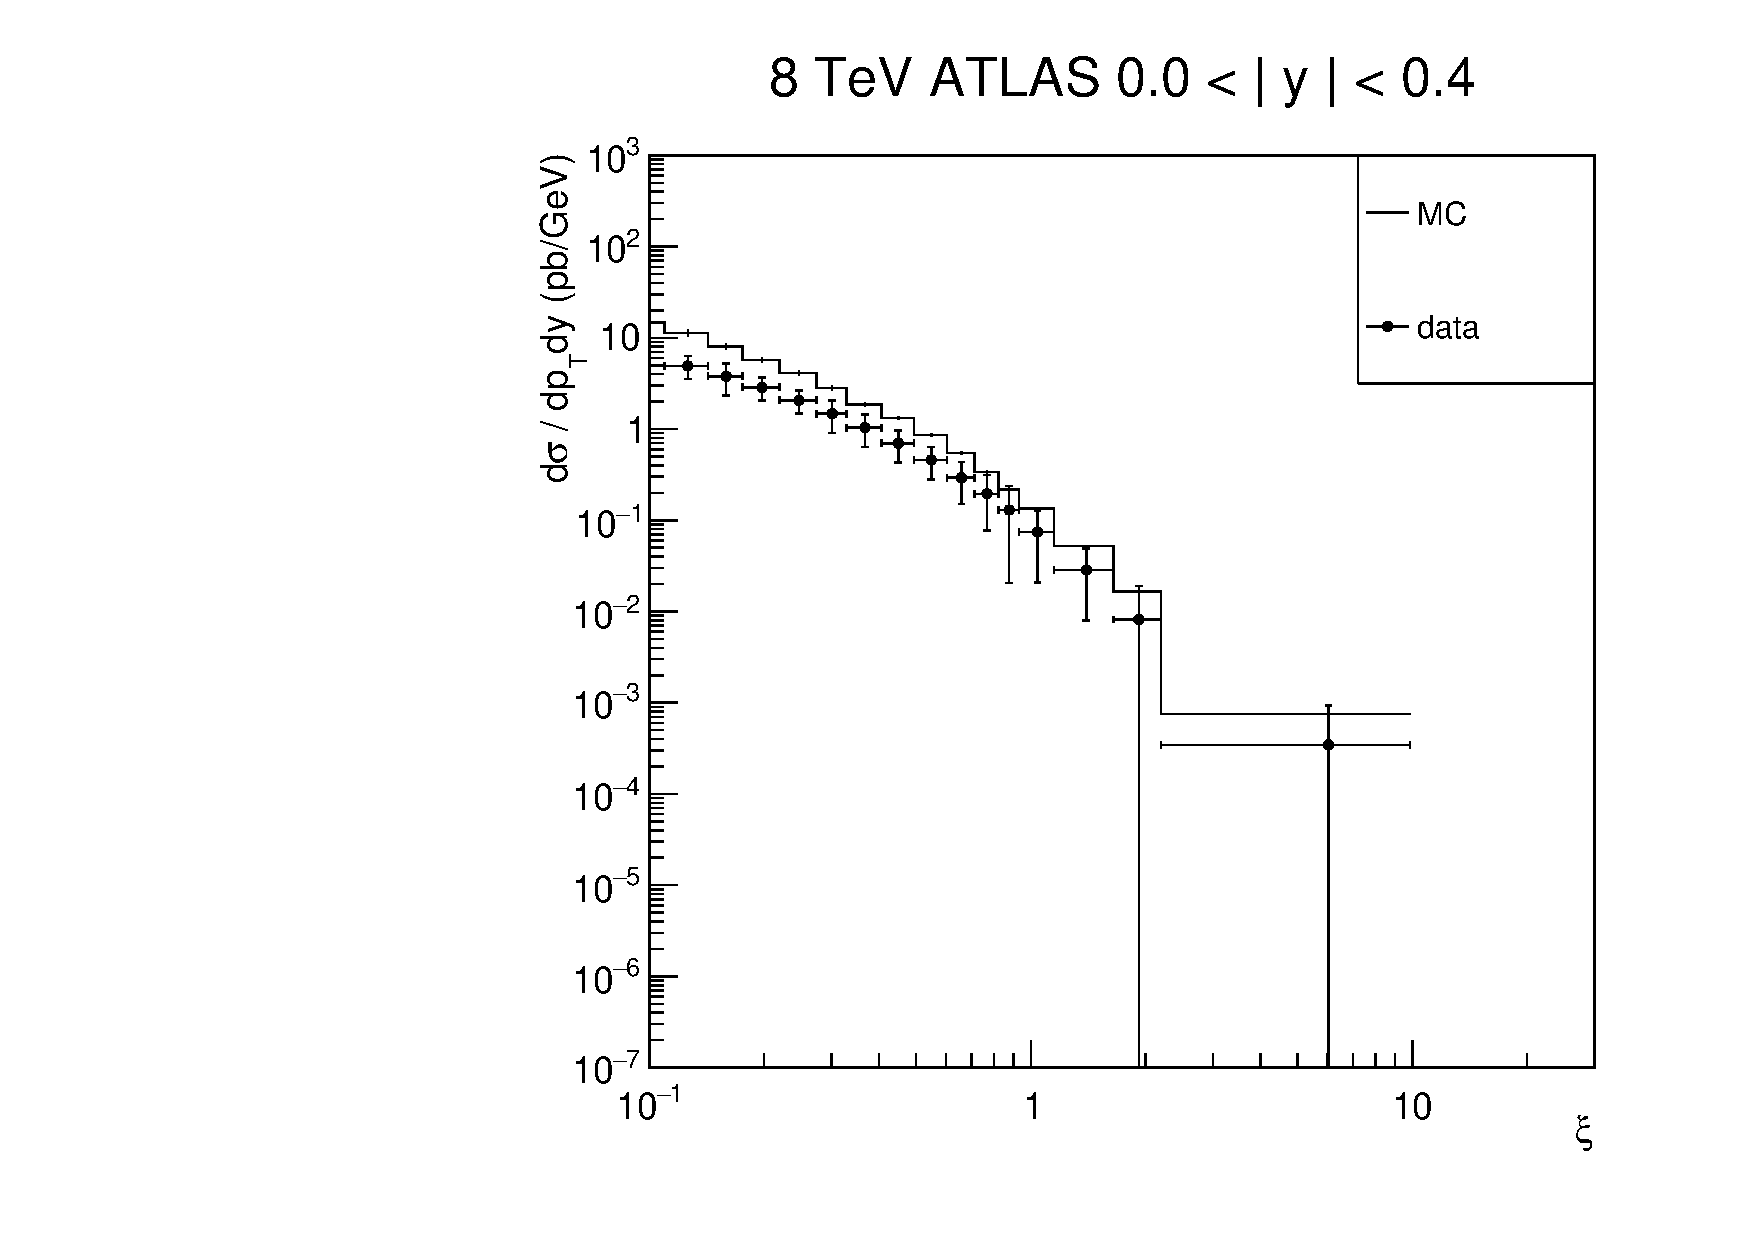
\includegraphics[width = 0.4\textwidth]{xi_8_A_y1.pdf}
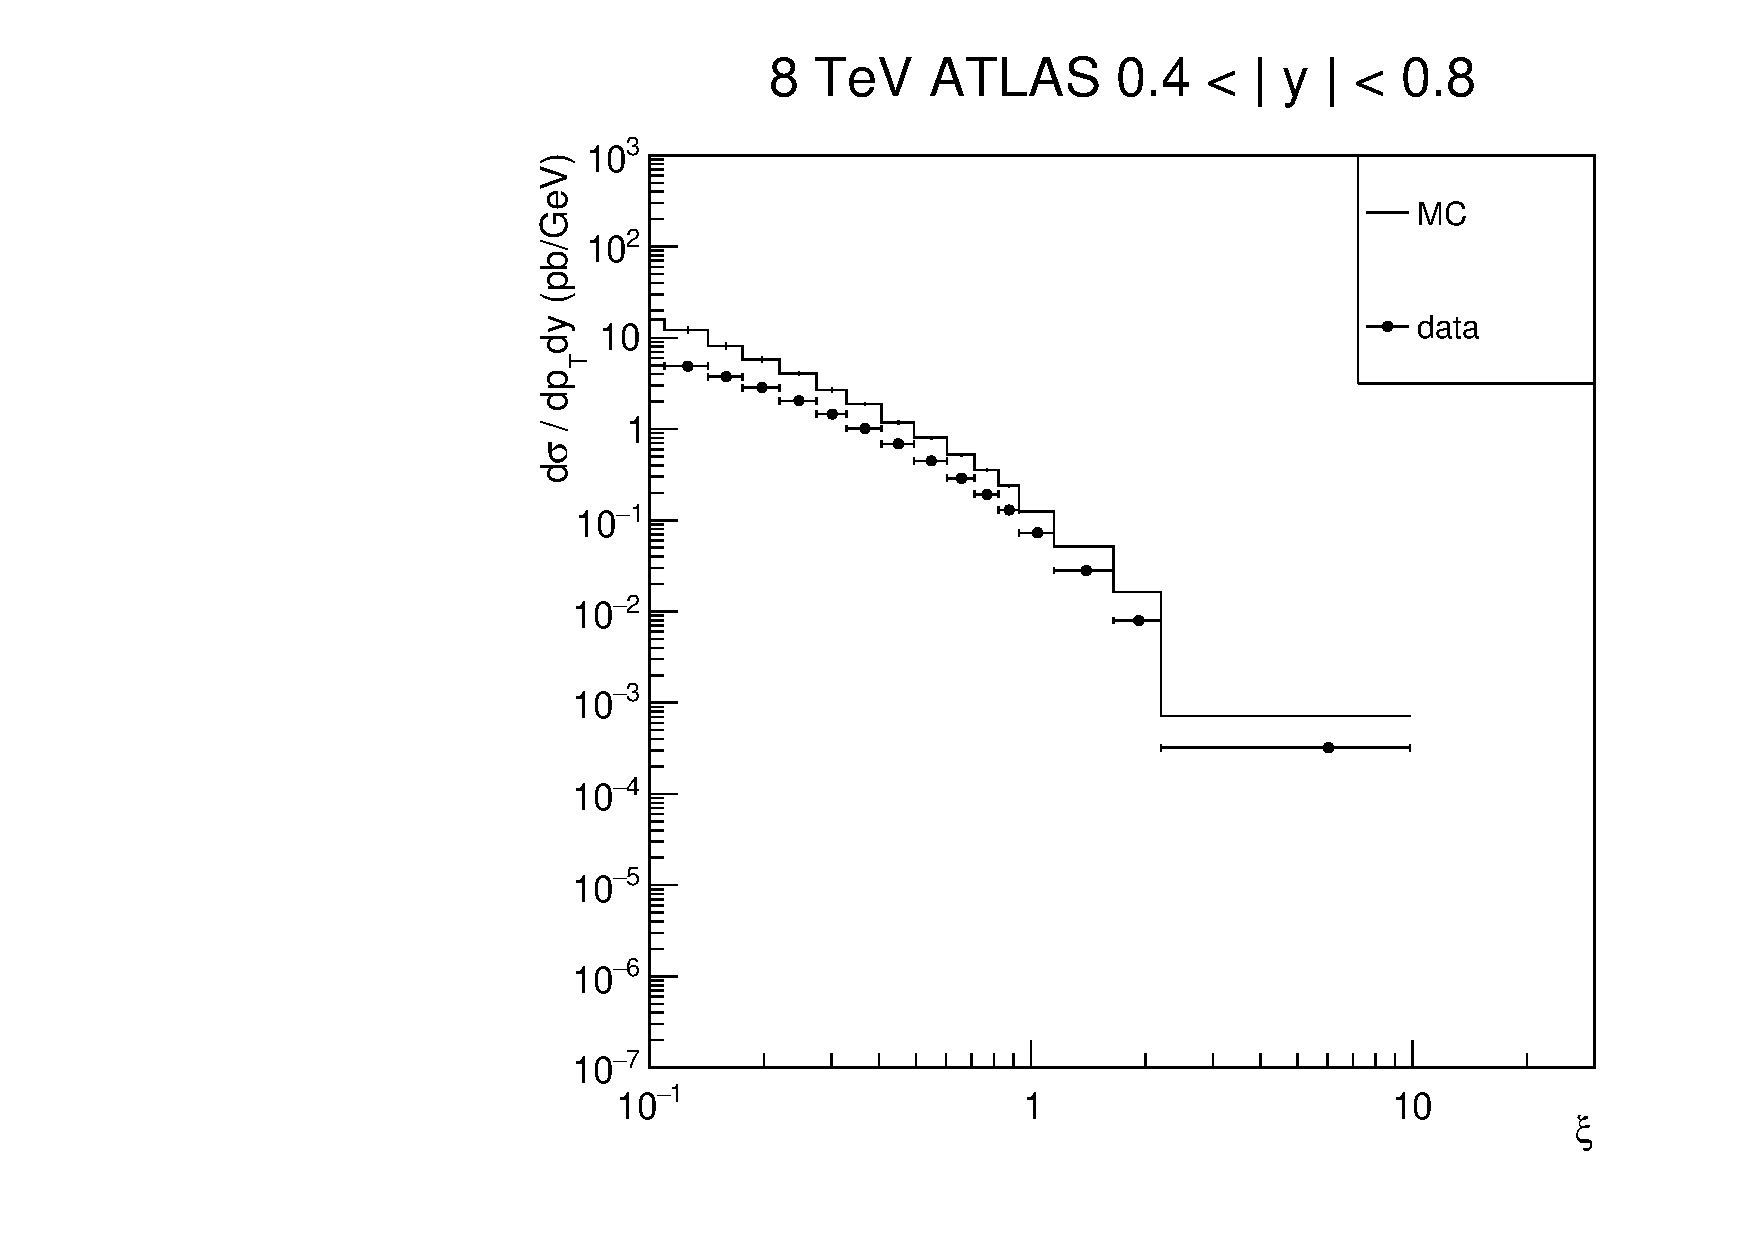
\includegraphics[width = 0.4\textwidth]{xi_8_A_y2.pdf}

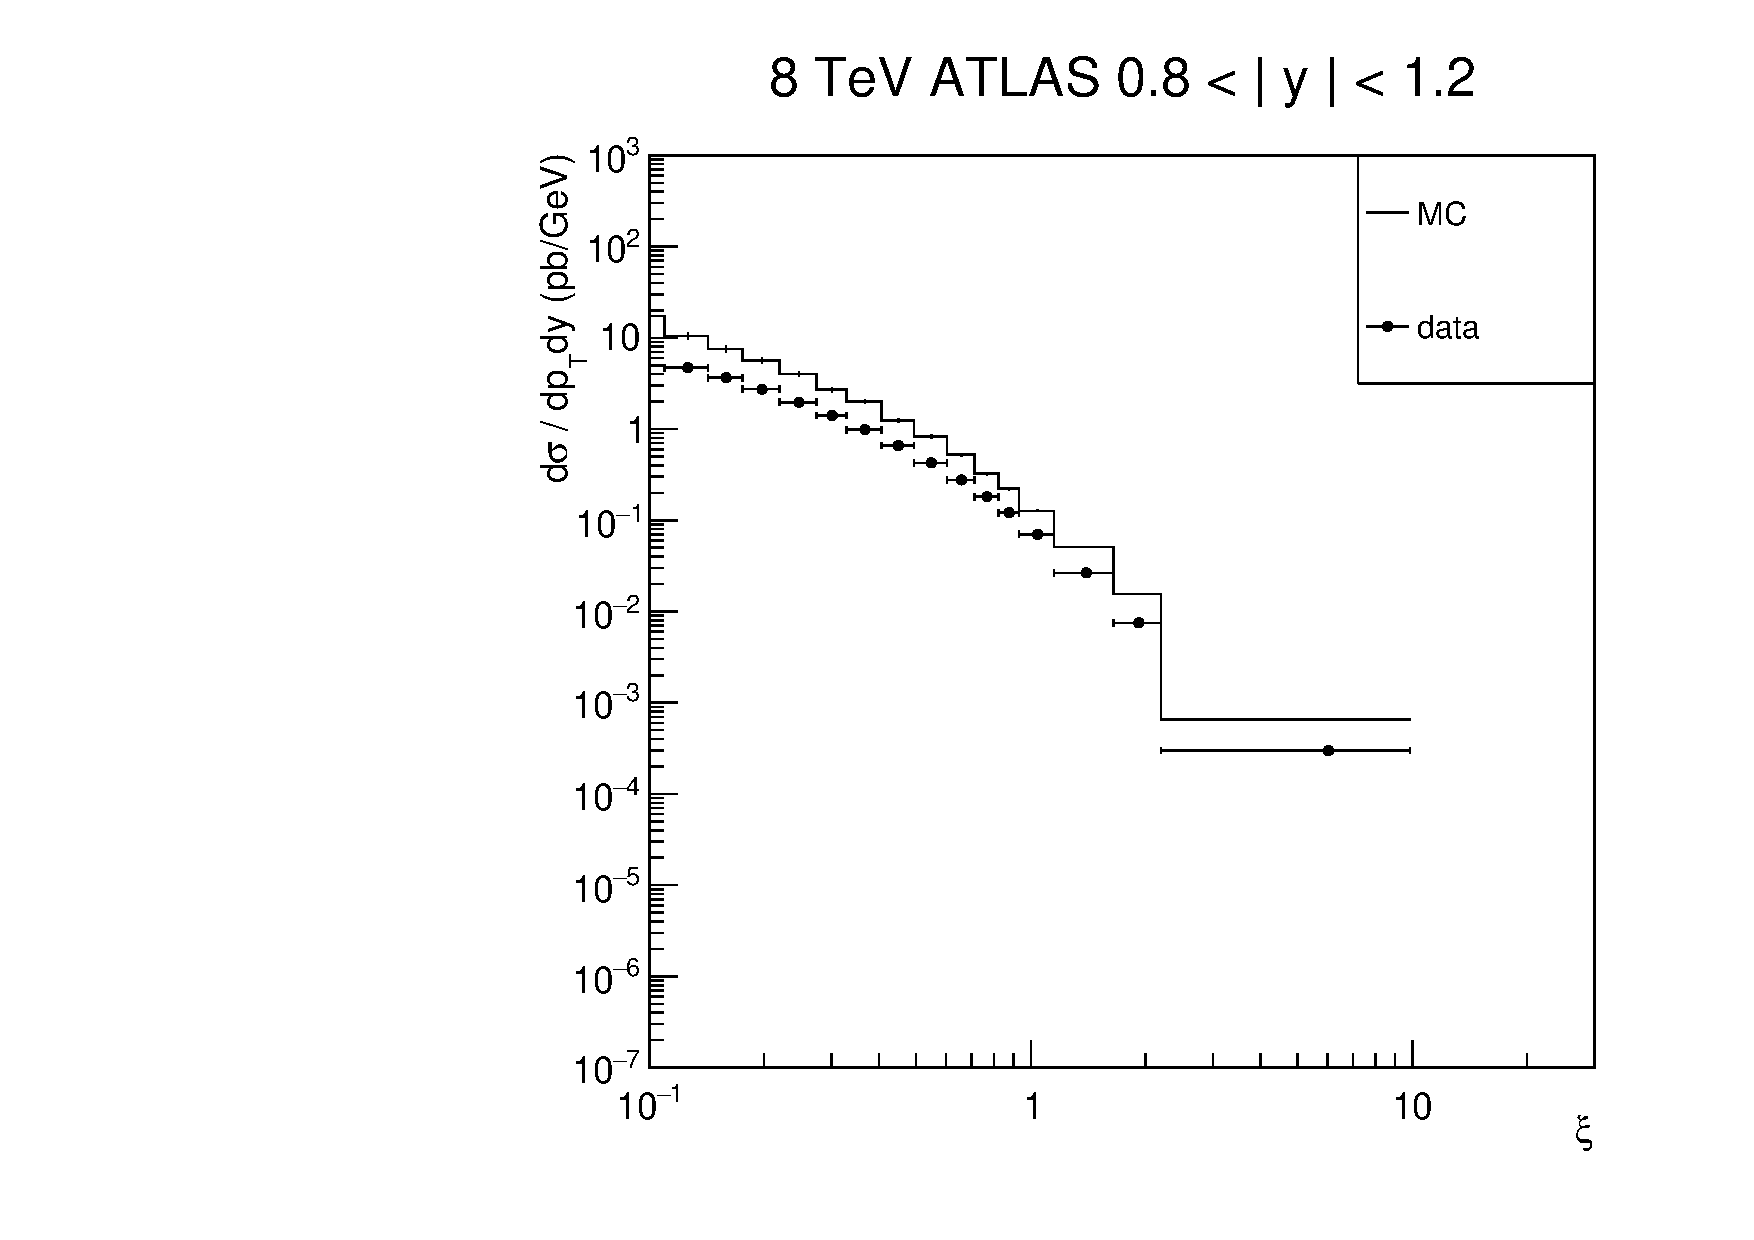
\includegraphics[width = 0.4\textwidth]{xi_8_A_y3.pdf}
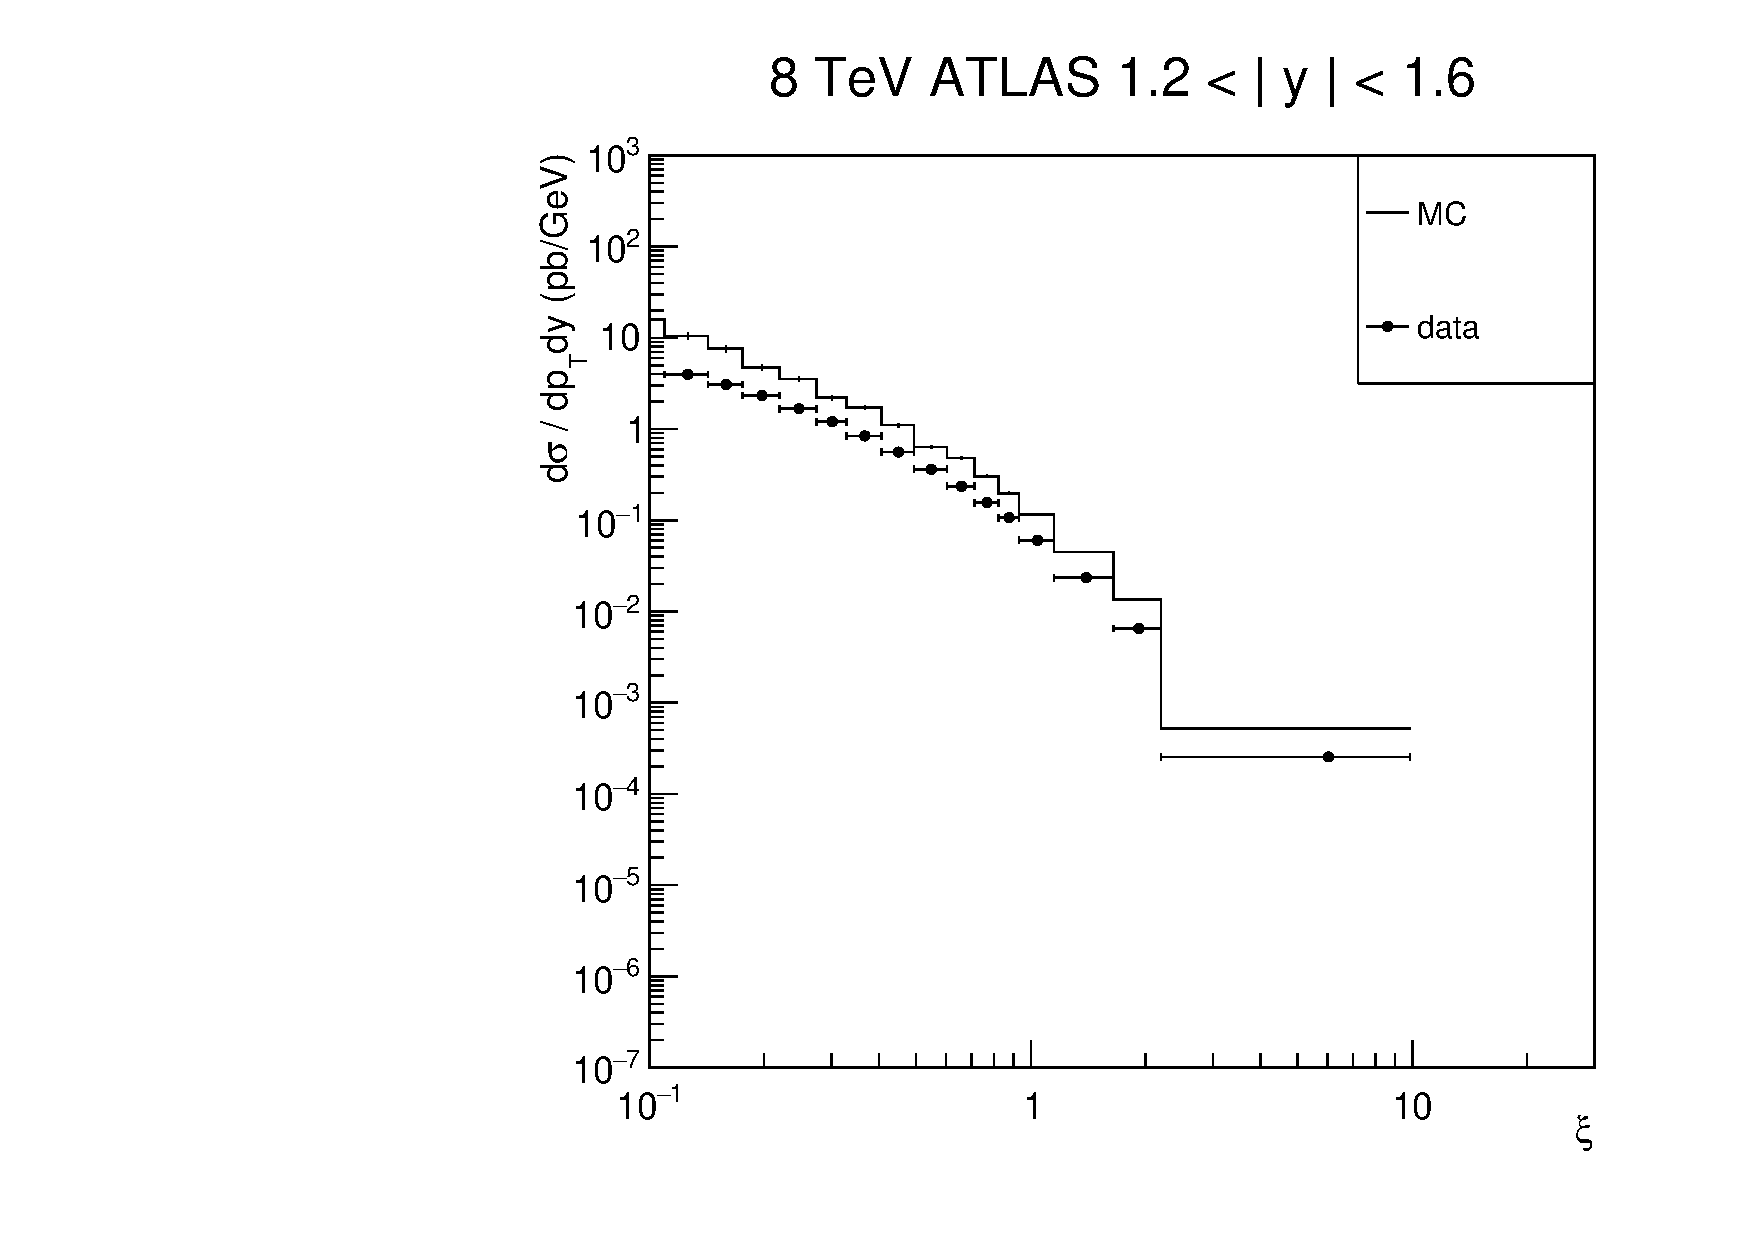
\includegraphics[width = 0.4\textwidth]{xi_8_A_y4.pdf}

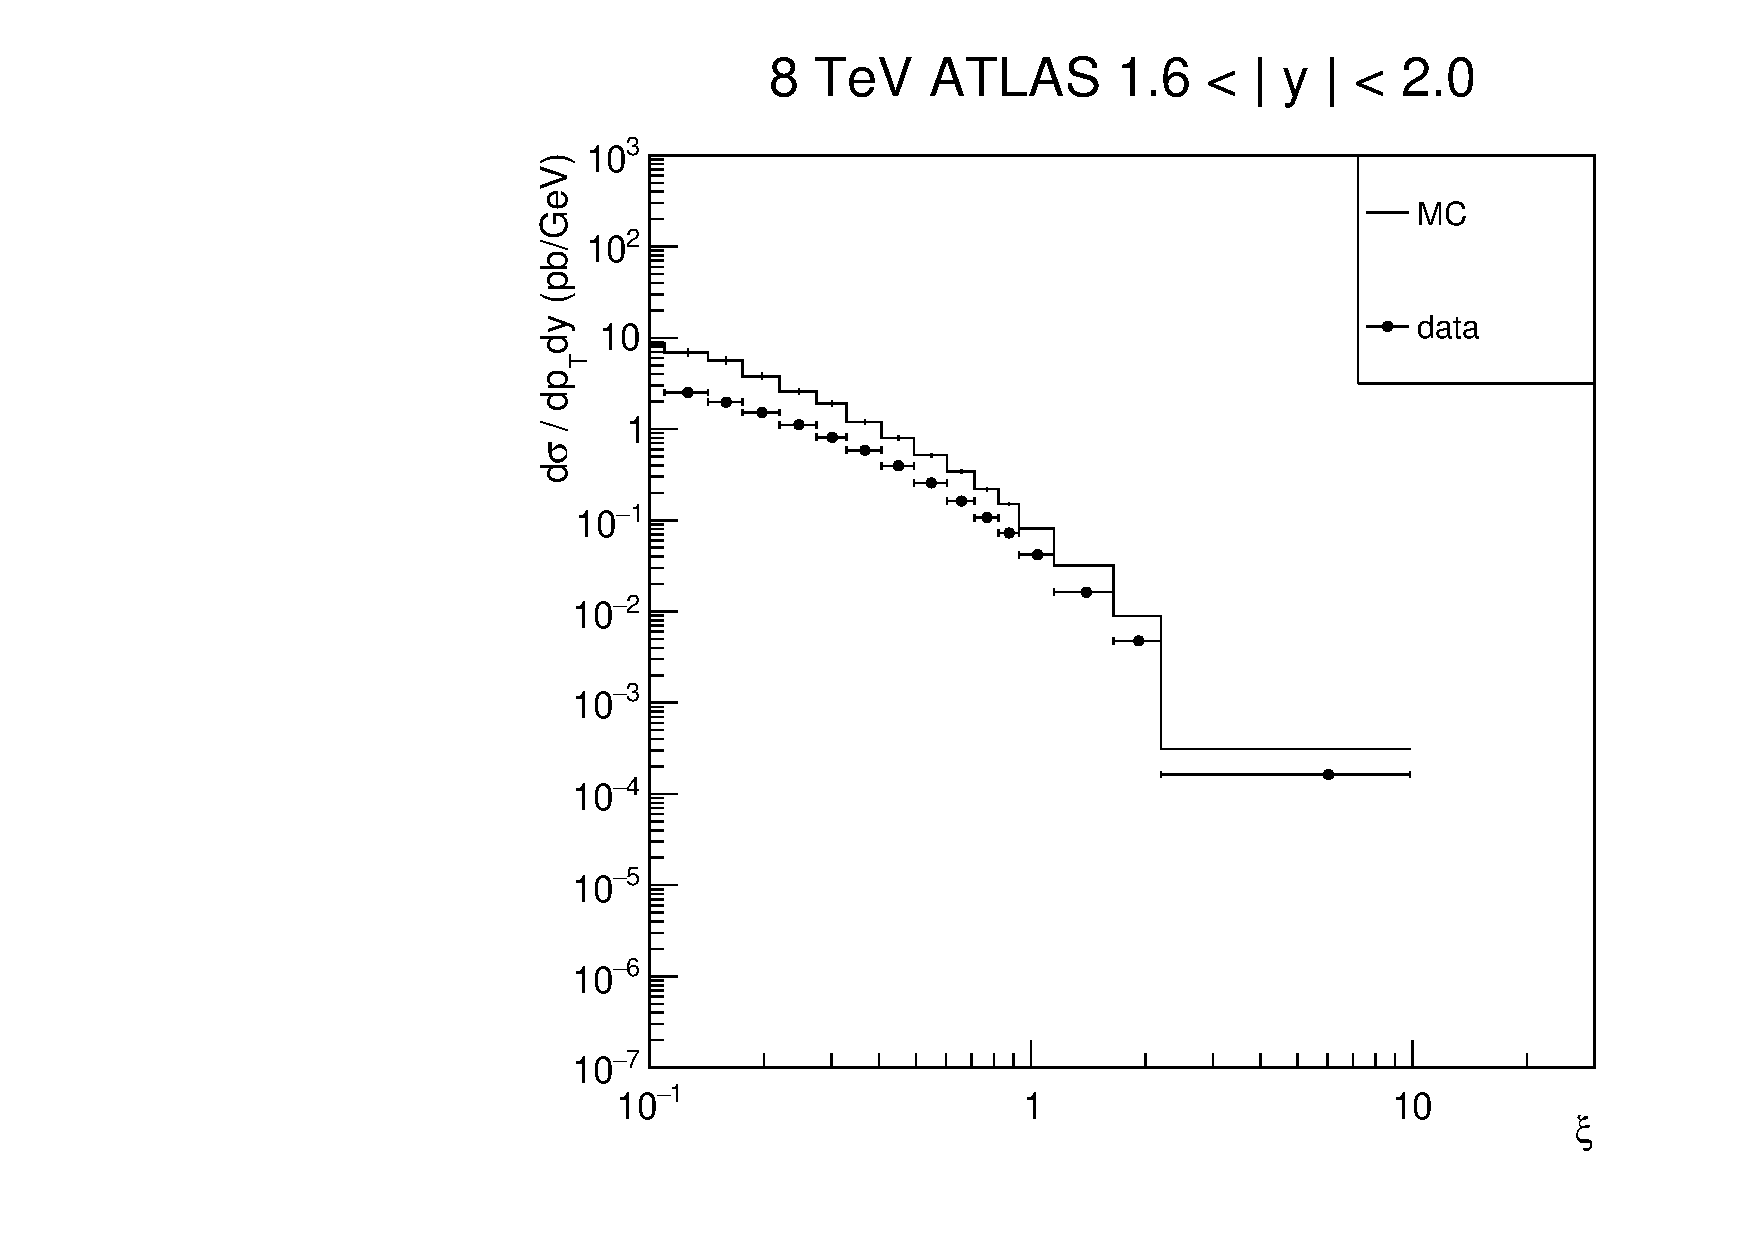
\includegraphics[width = 0.4\textwidth]{xi_8_A_y5.pdf}
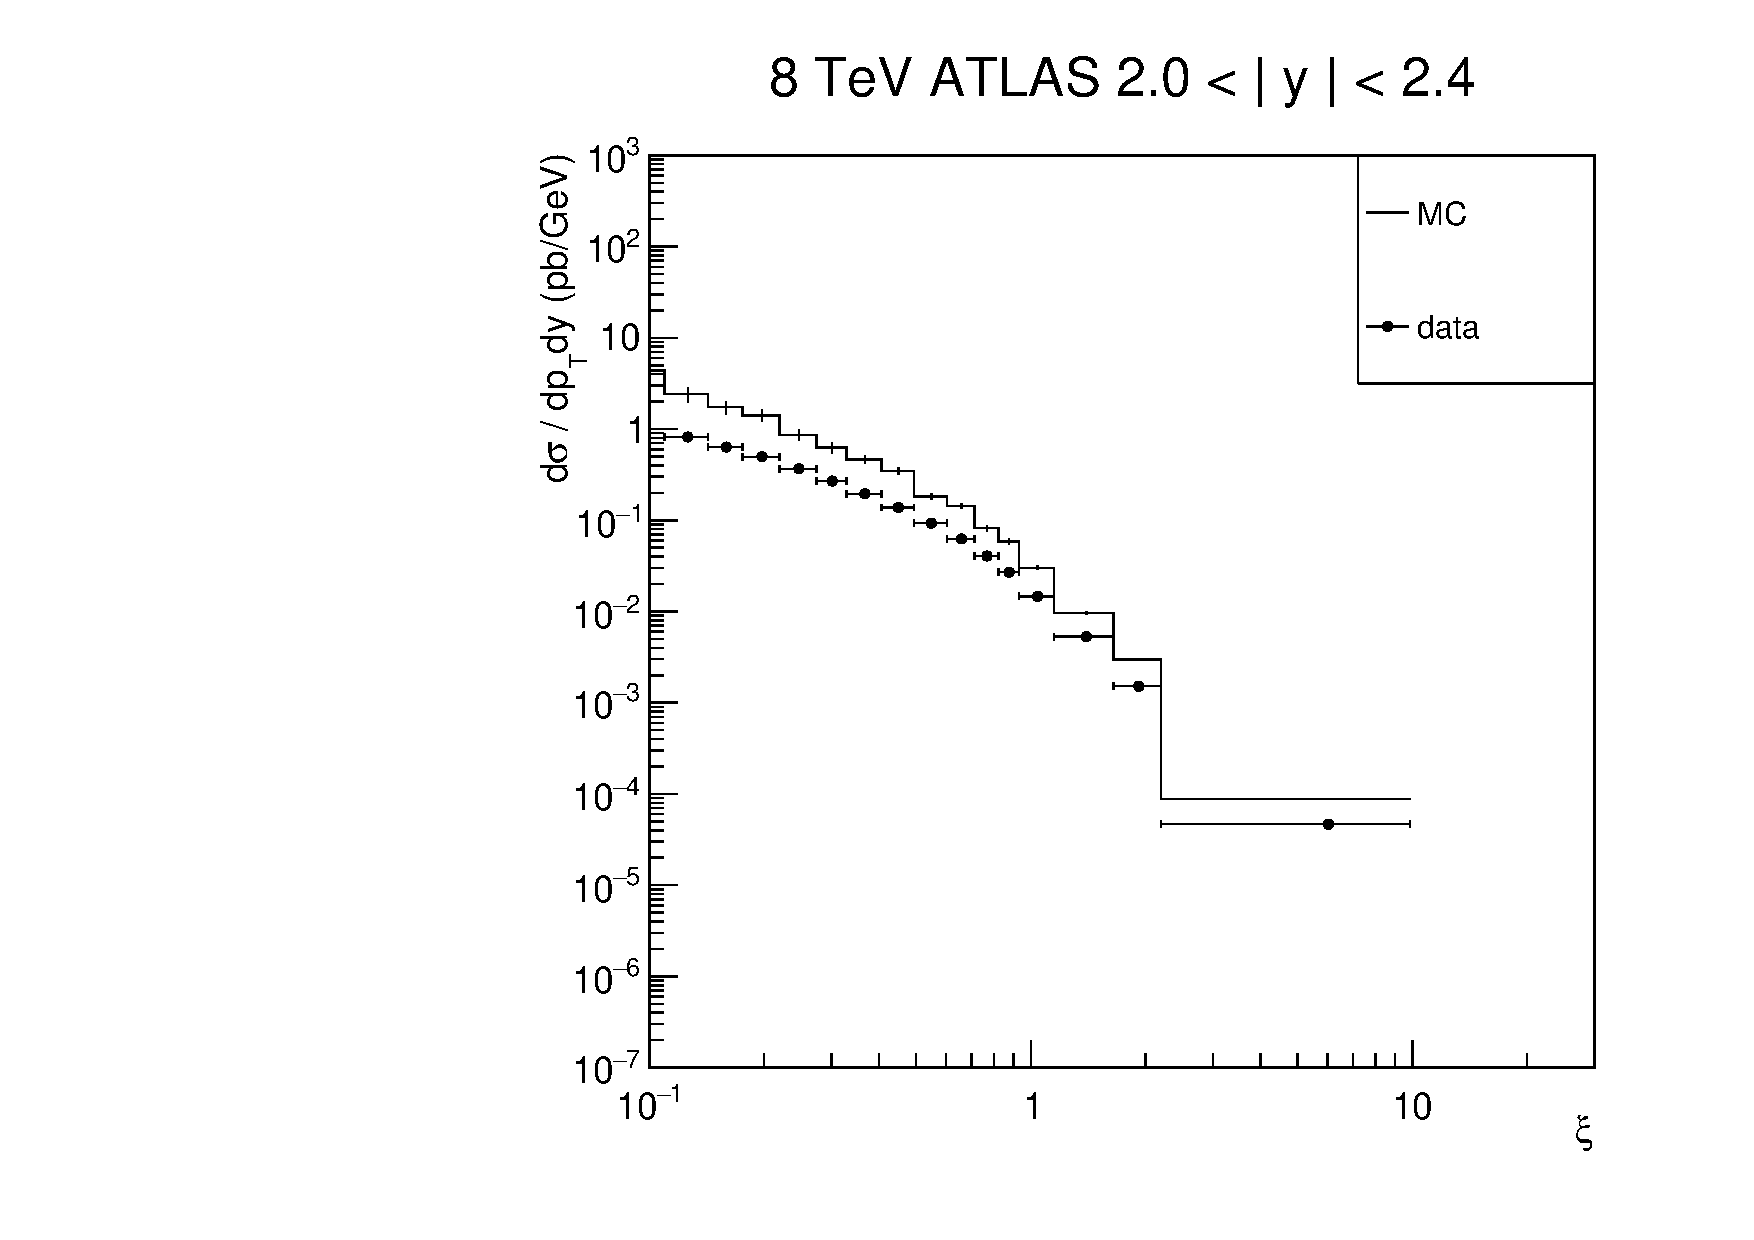
\includegraphics[width = 0.4\textwidth]{xi_8_A_y6.pdf}
%\caption{Comparison between MC $\xi$ distribution and data points in the six $y$ bins of the data, for 8 TeV. All histograms divided by total nr events and multiplied by same normalization factor. Data is not scaled.}\label{f:xi_comp}
\end{figure}

\clearpage

\begin{figure}[h!]
\centering
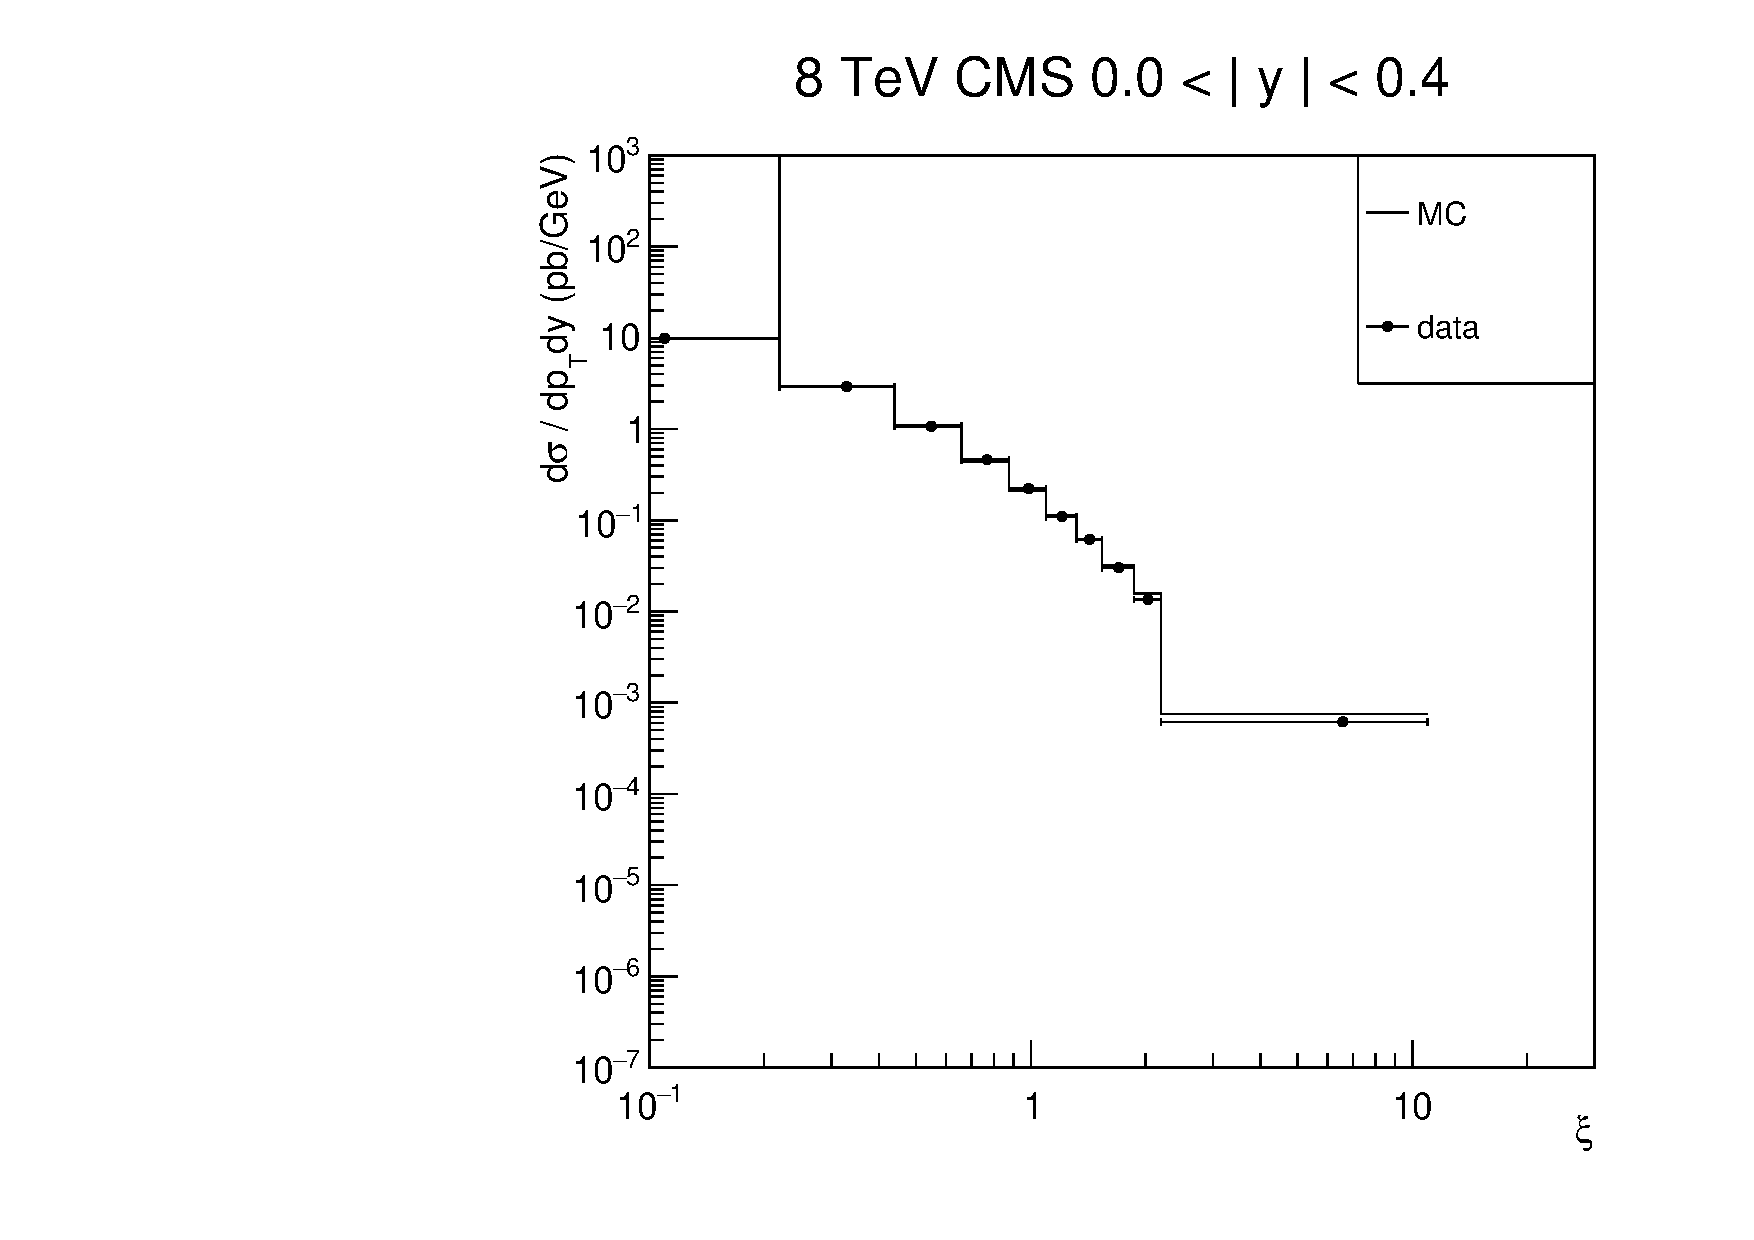
\includegraphics[width = 0.4\textwidth]{xi_8_C_y1.pdf}
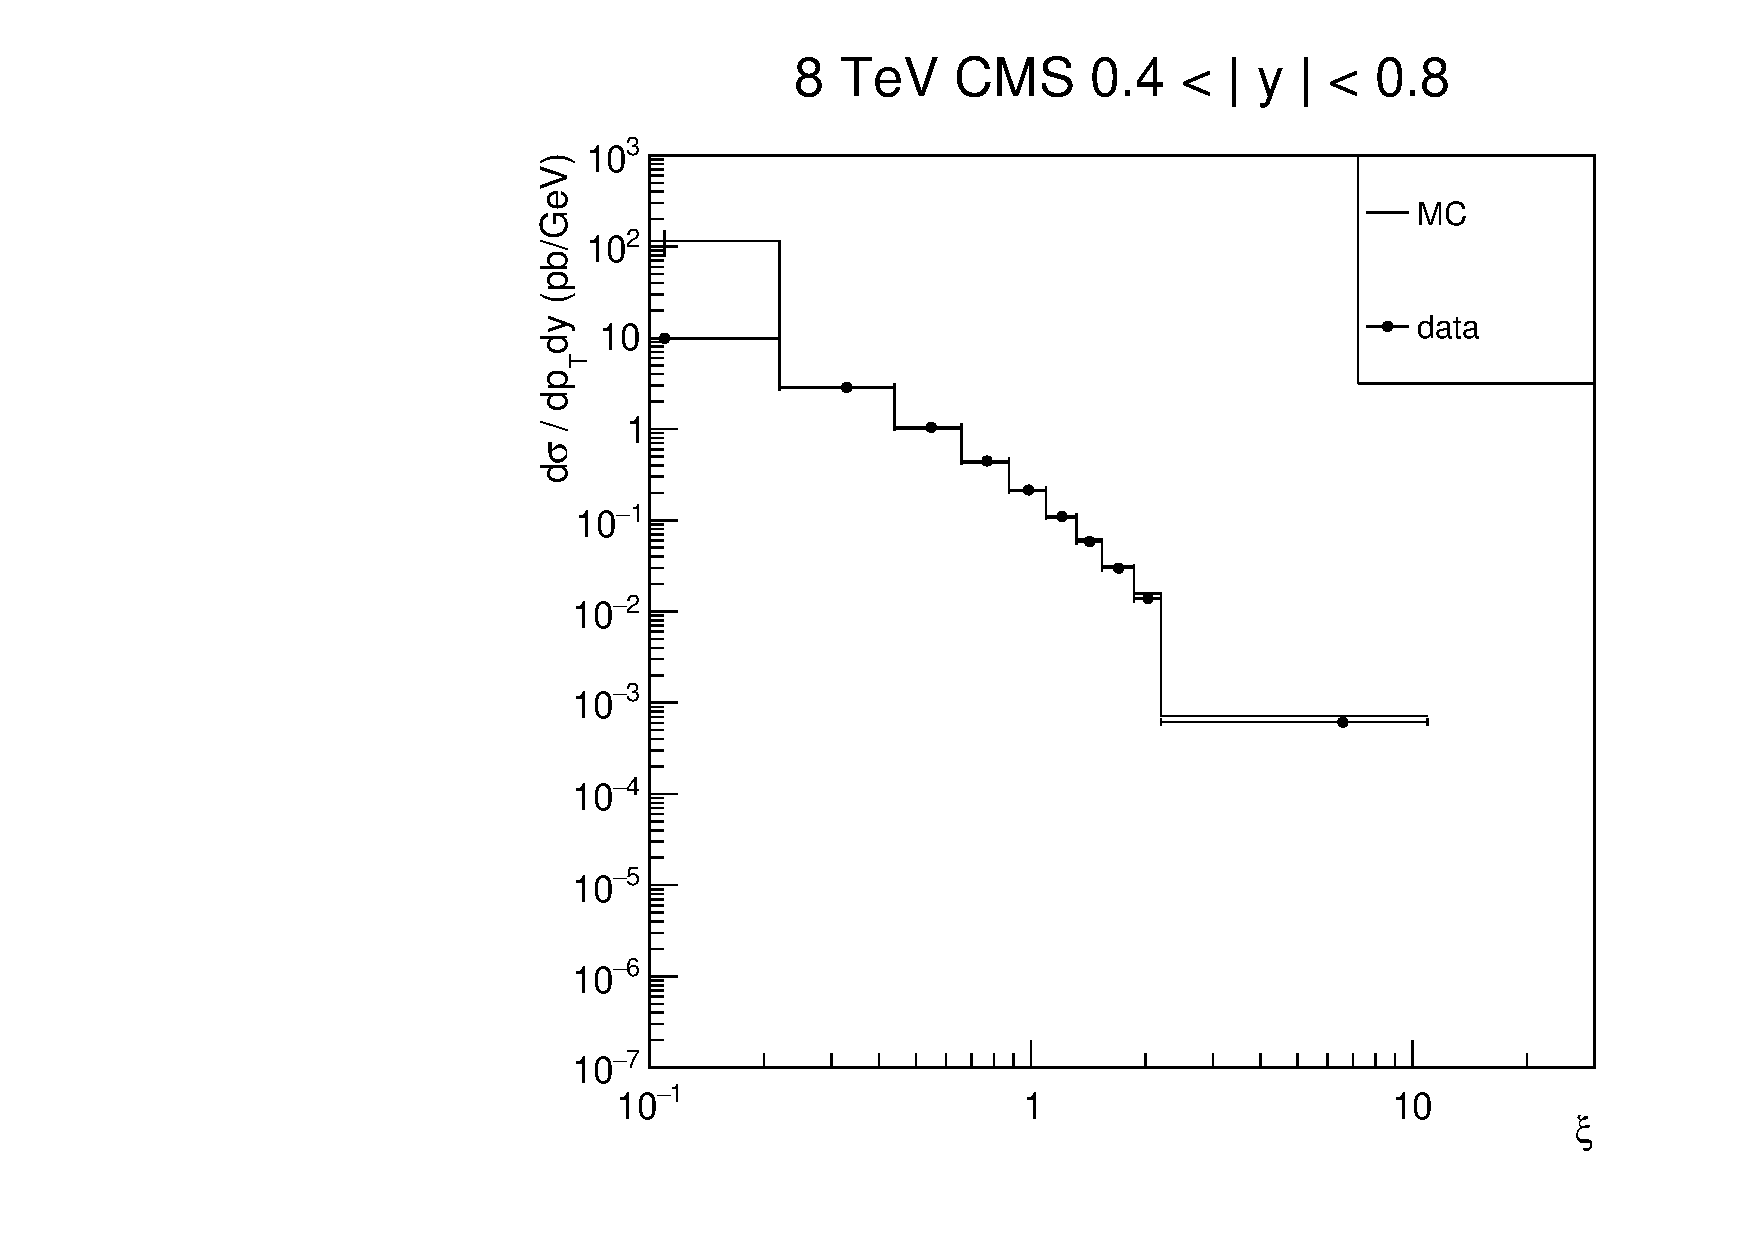
\includegraphics[width = 0.4\textwidth]{xi_8_C_y2.pdf}

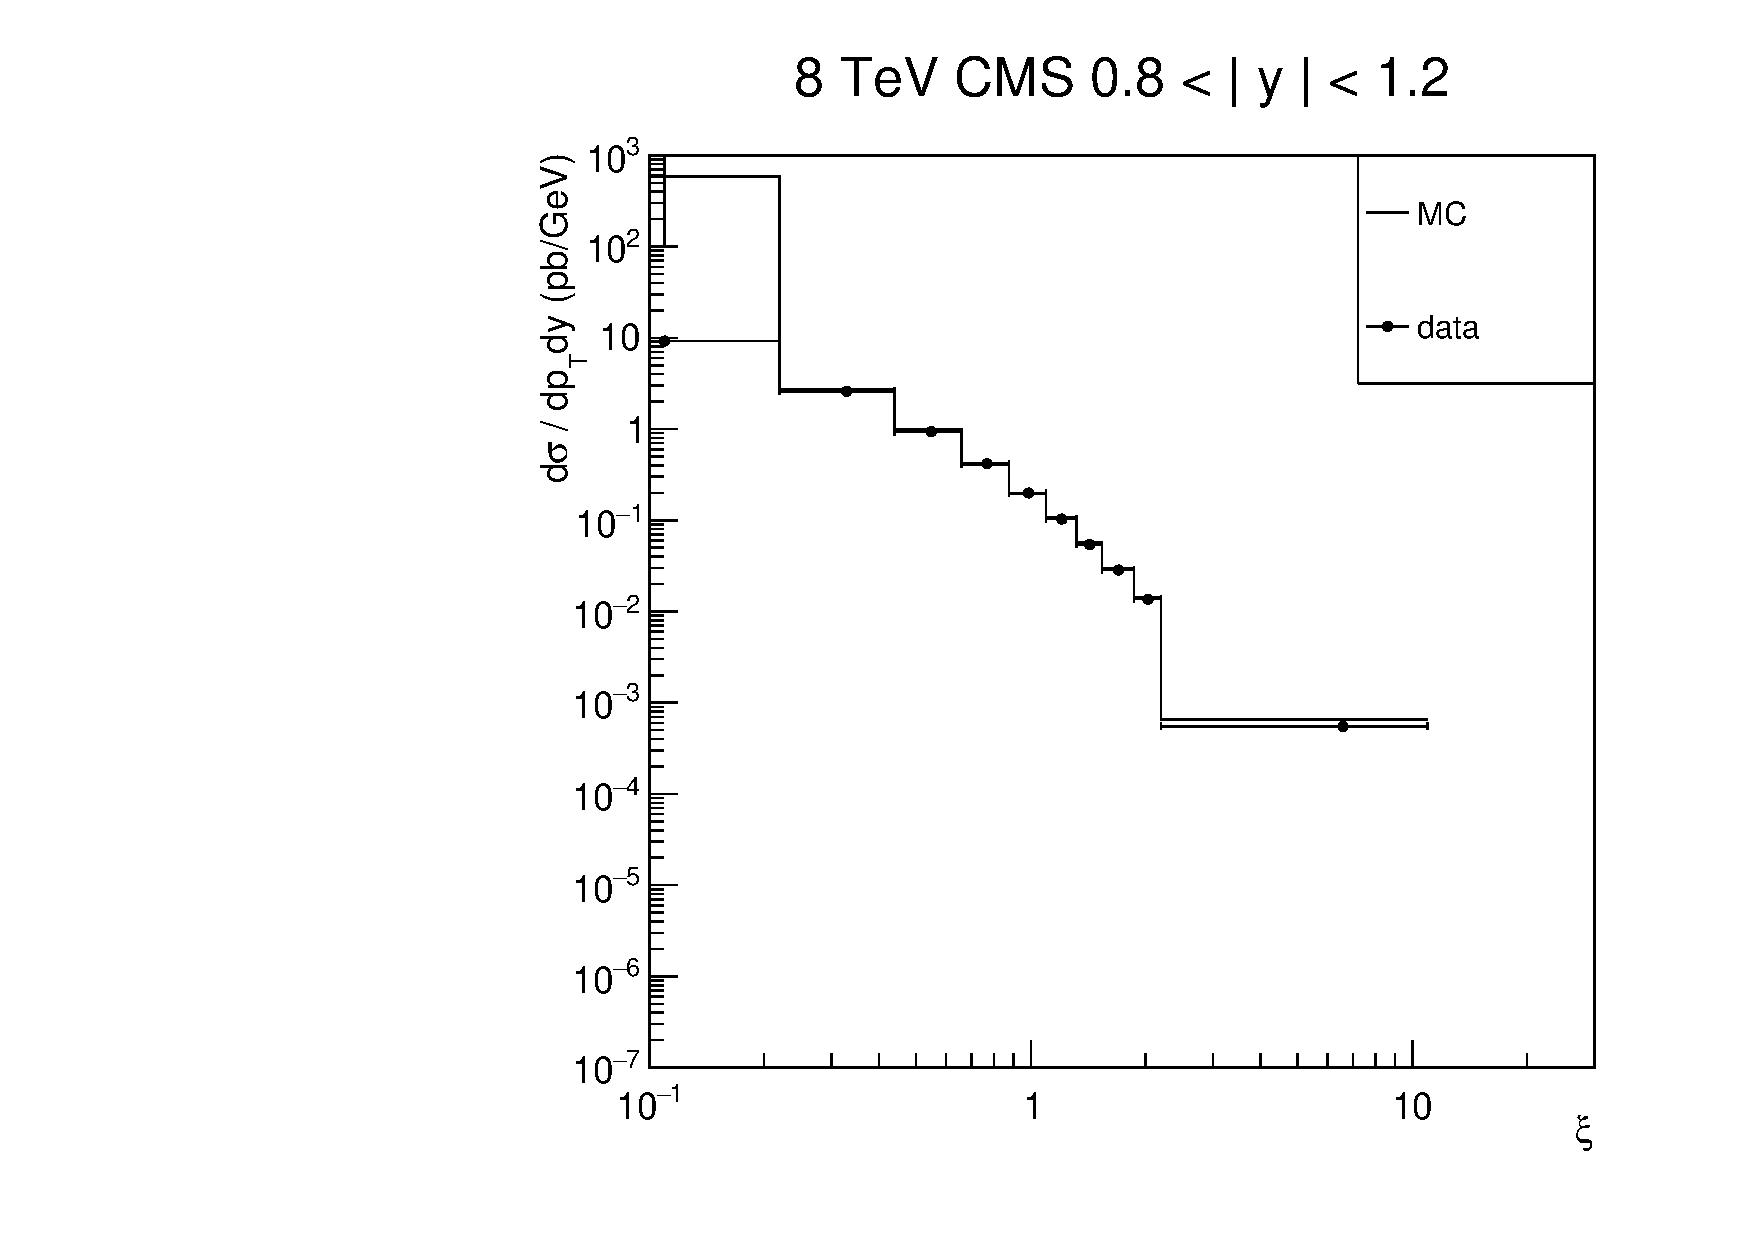
\includegraphics[width = 0.4\textwidth]{xi_8_C_y3.pdf}
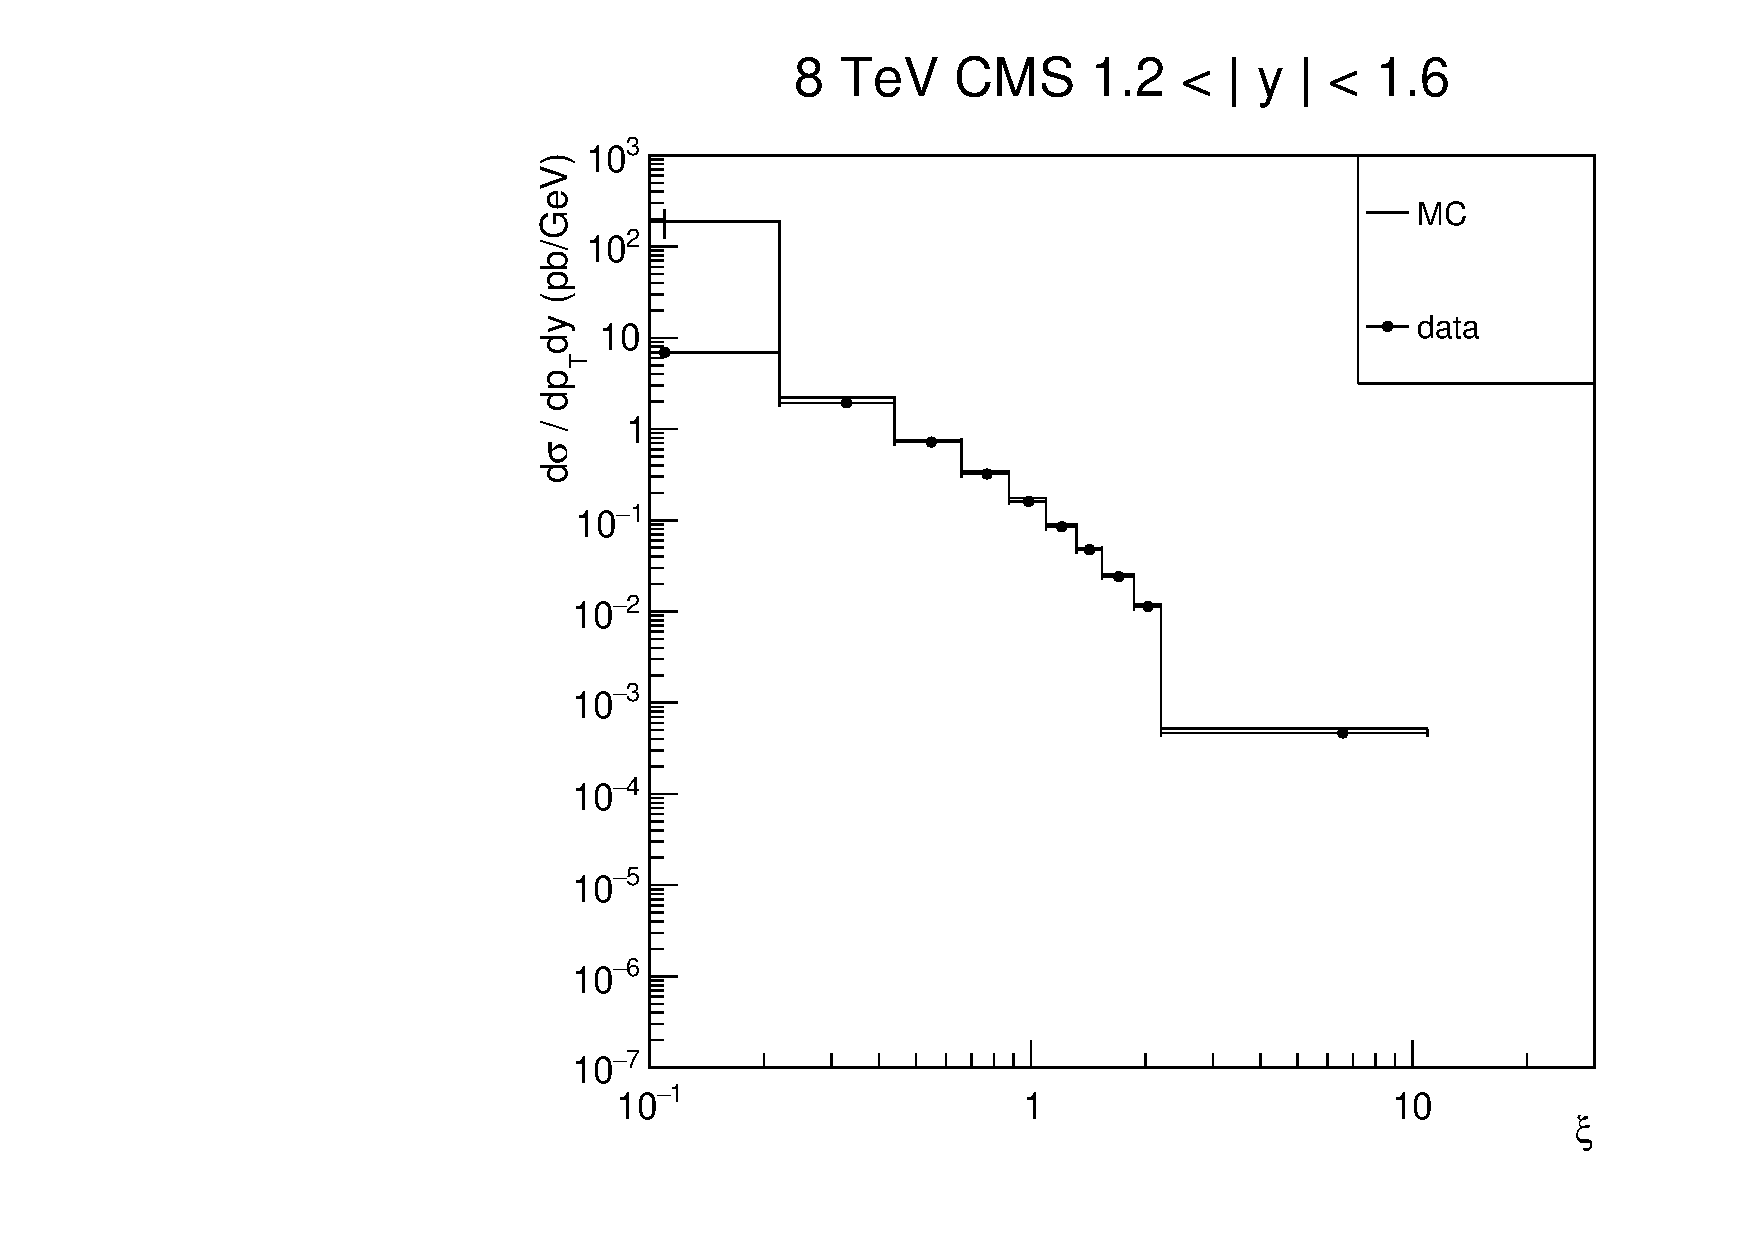
\includegraphics[width = 0.4\textwidth]{xi_8_C_y4.pdf}

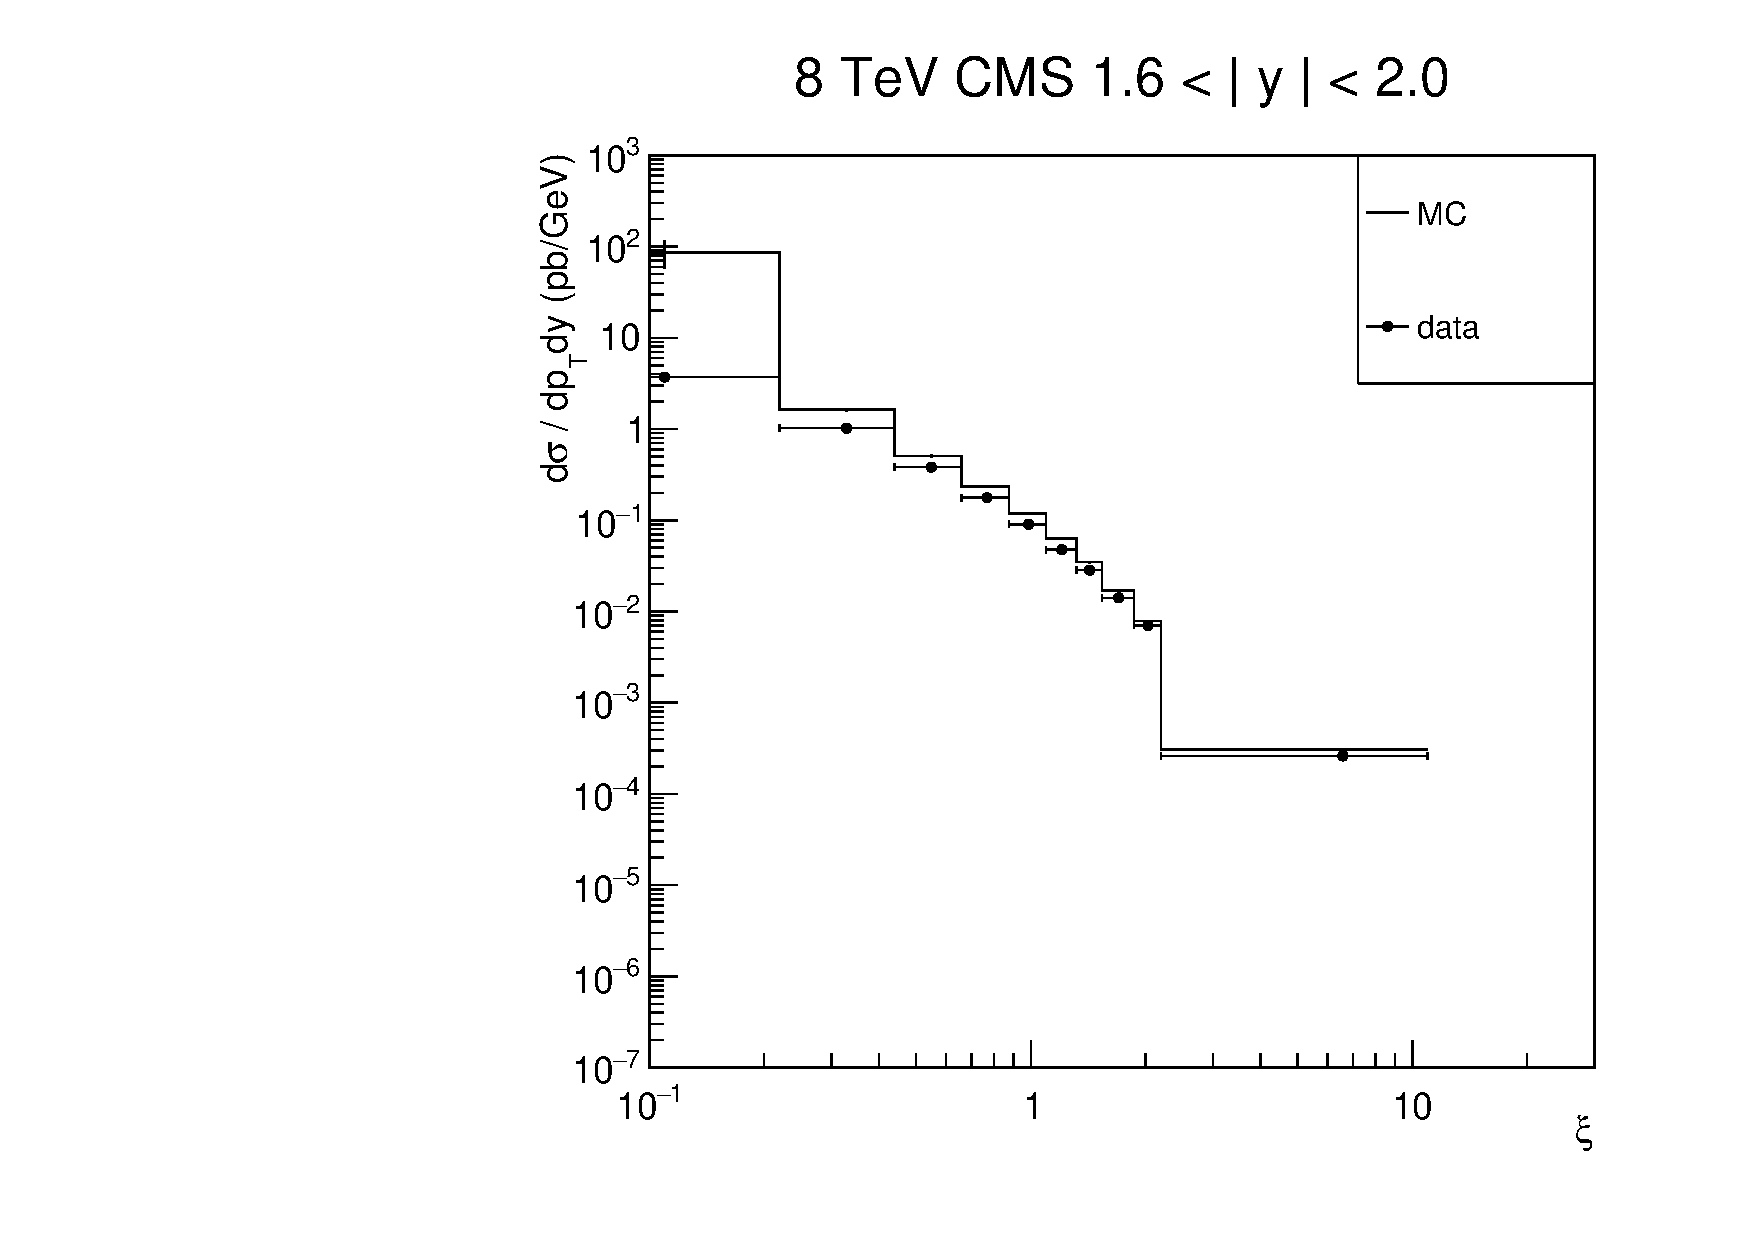
\includegraphics[width = 0.4\textwidth]{xi_8_C_y5.pdf}
%\caption{Comparison between MC $\xi$ distribution and data points in the six $y$ bins of the data, for 8 TeV. All histograms divided by total nr events and multiplied by same normalization factor. Data is not scaled.}\label{f:xi_comp}
\end{figure}

\clearpage

\begin{figure}[h!]
\centering
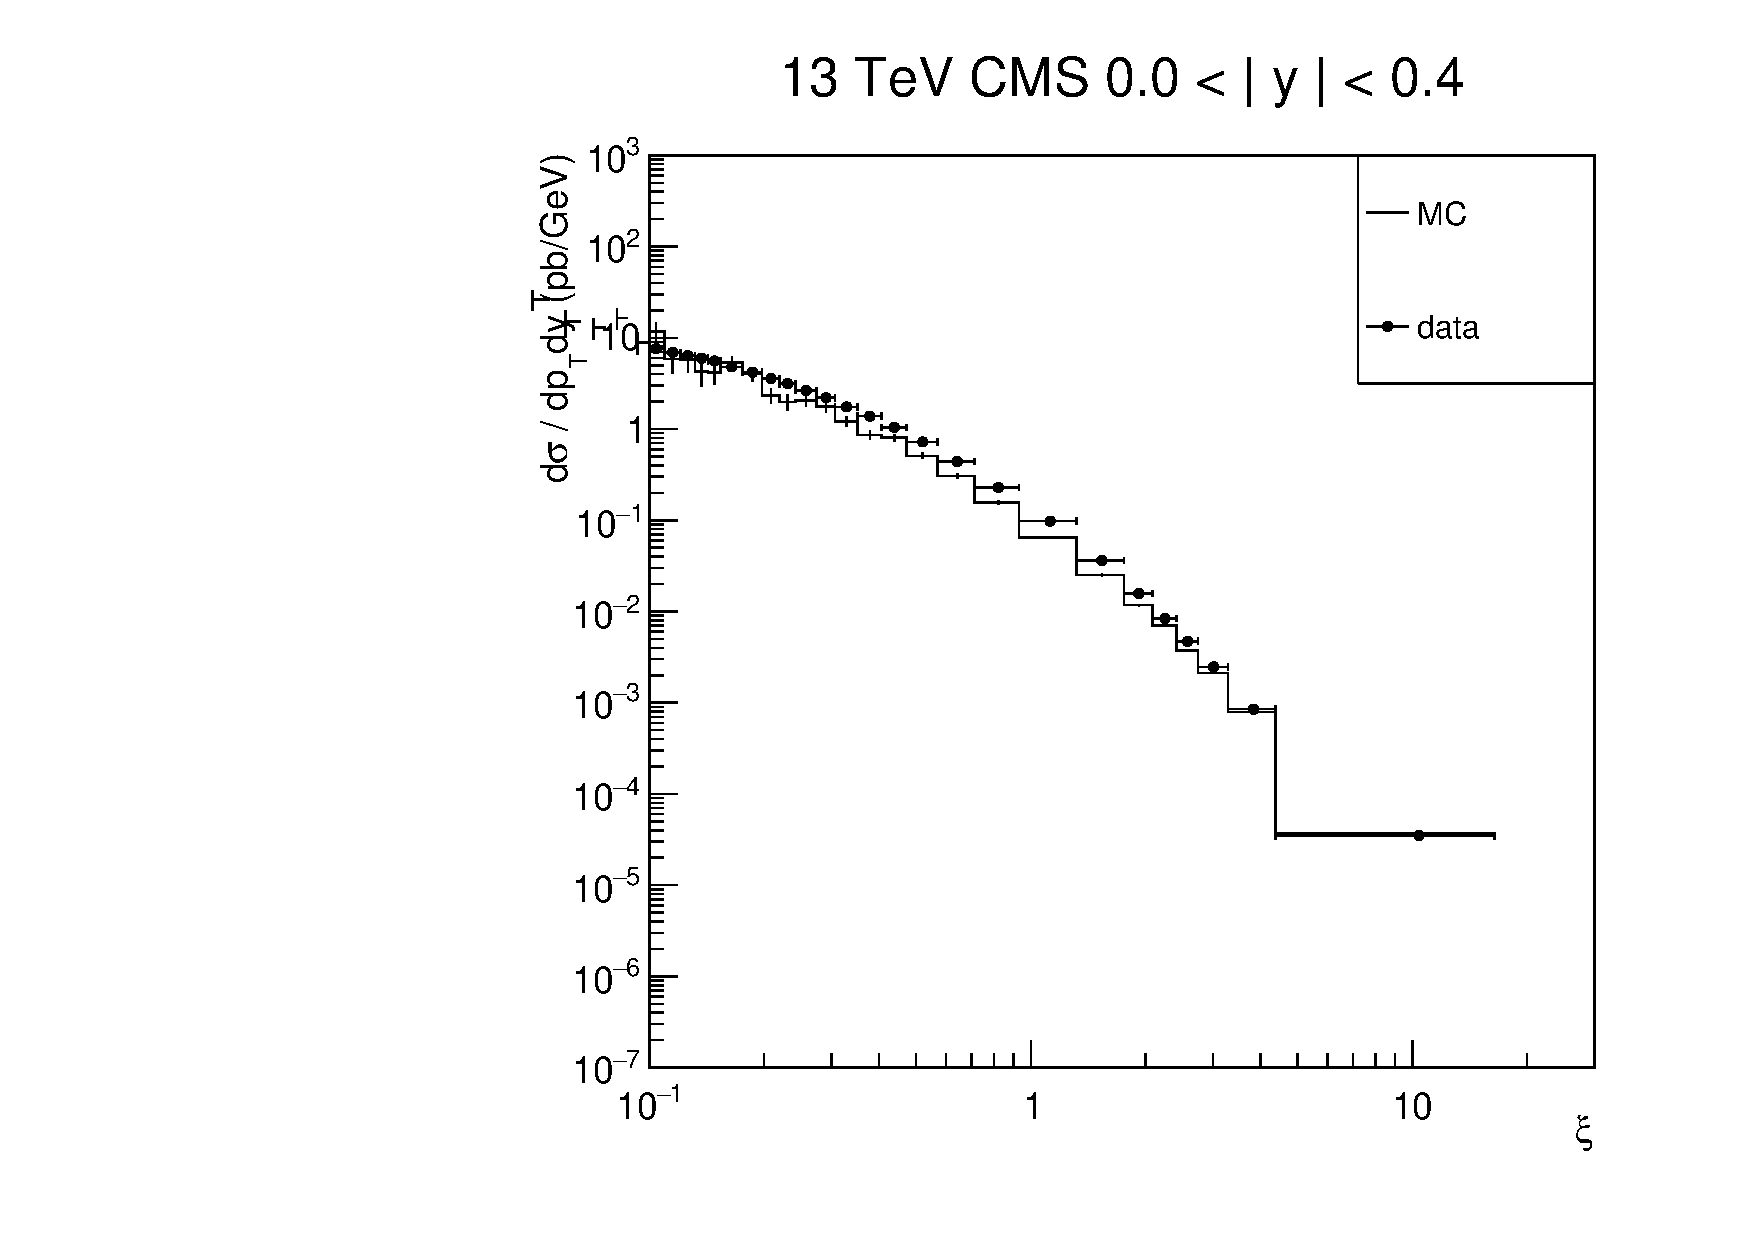
\includegraphics[width = 0.4\textwidth]{xi_13_C_y1.pdf}
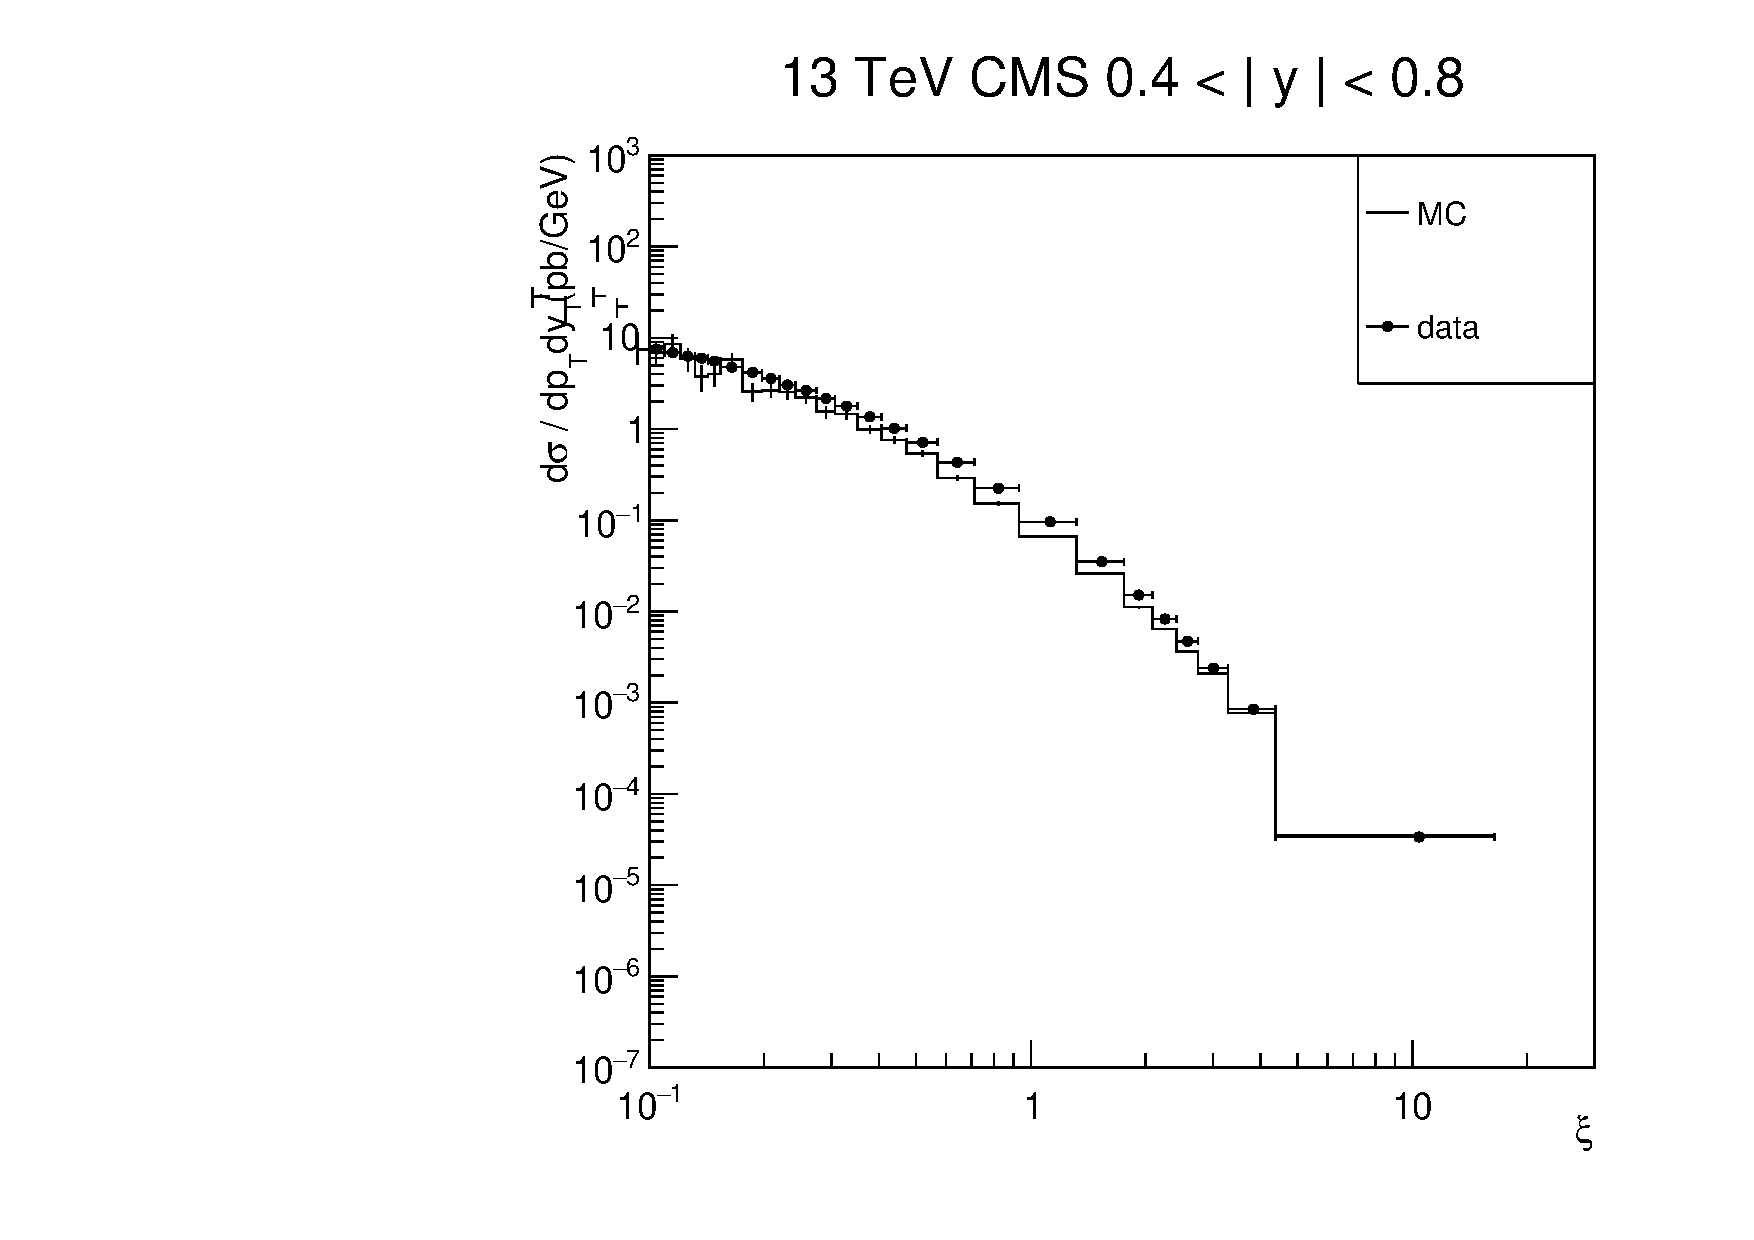
\includegraphics[width = 0.4\textwidth]{xi_13_C_y2.pdf}

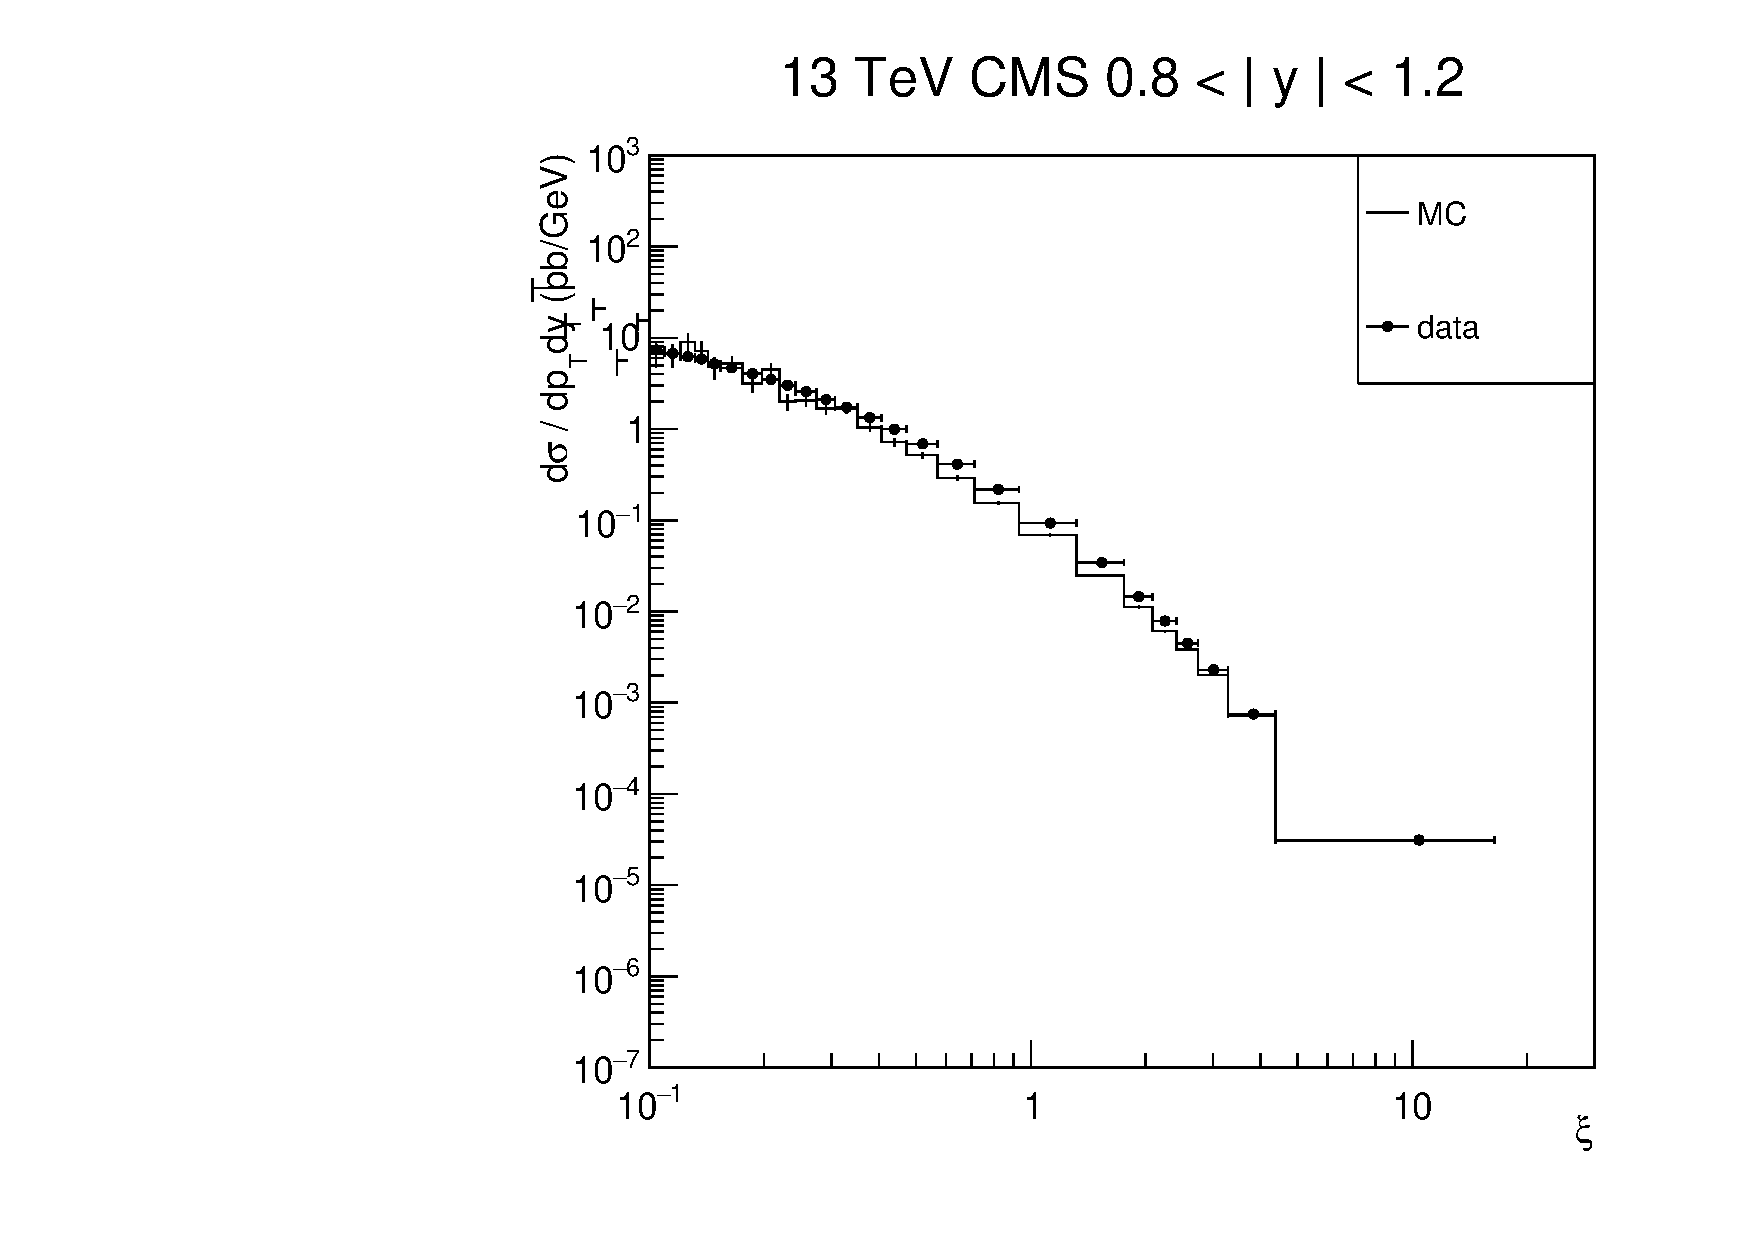
\includegraphics[width = 0.4\textwidth]{xi_13_C_y3.pdf}
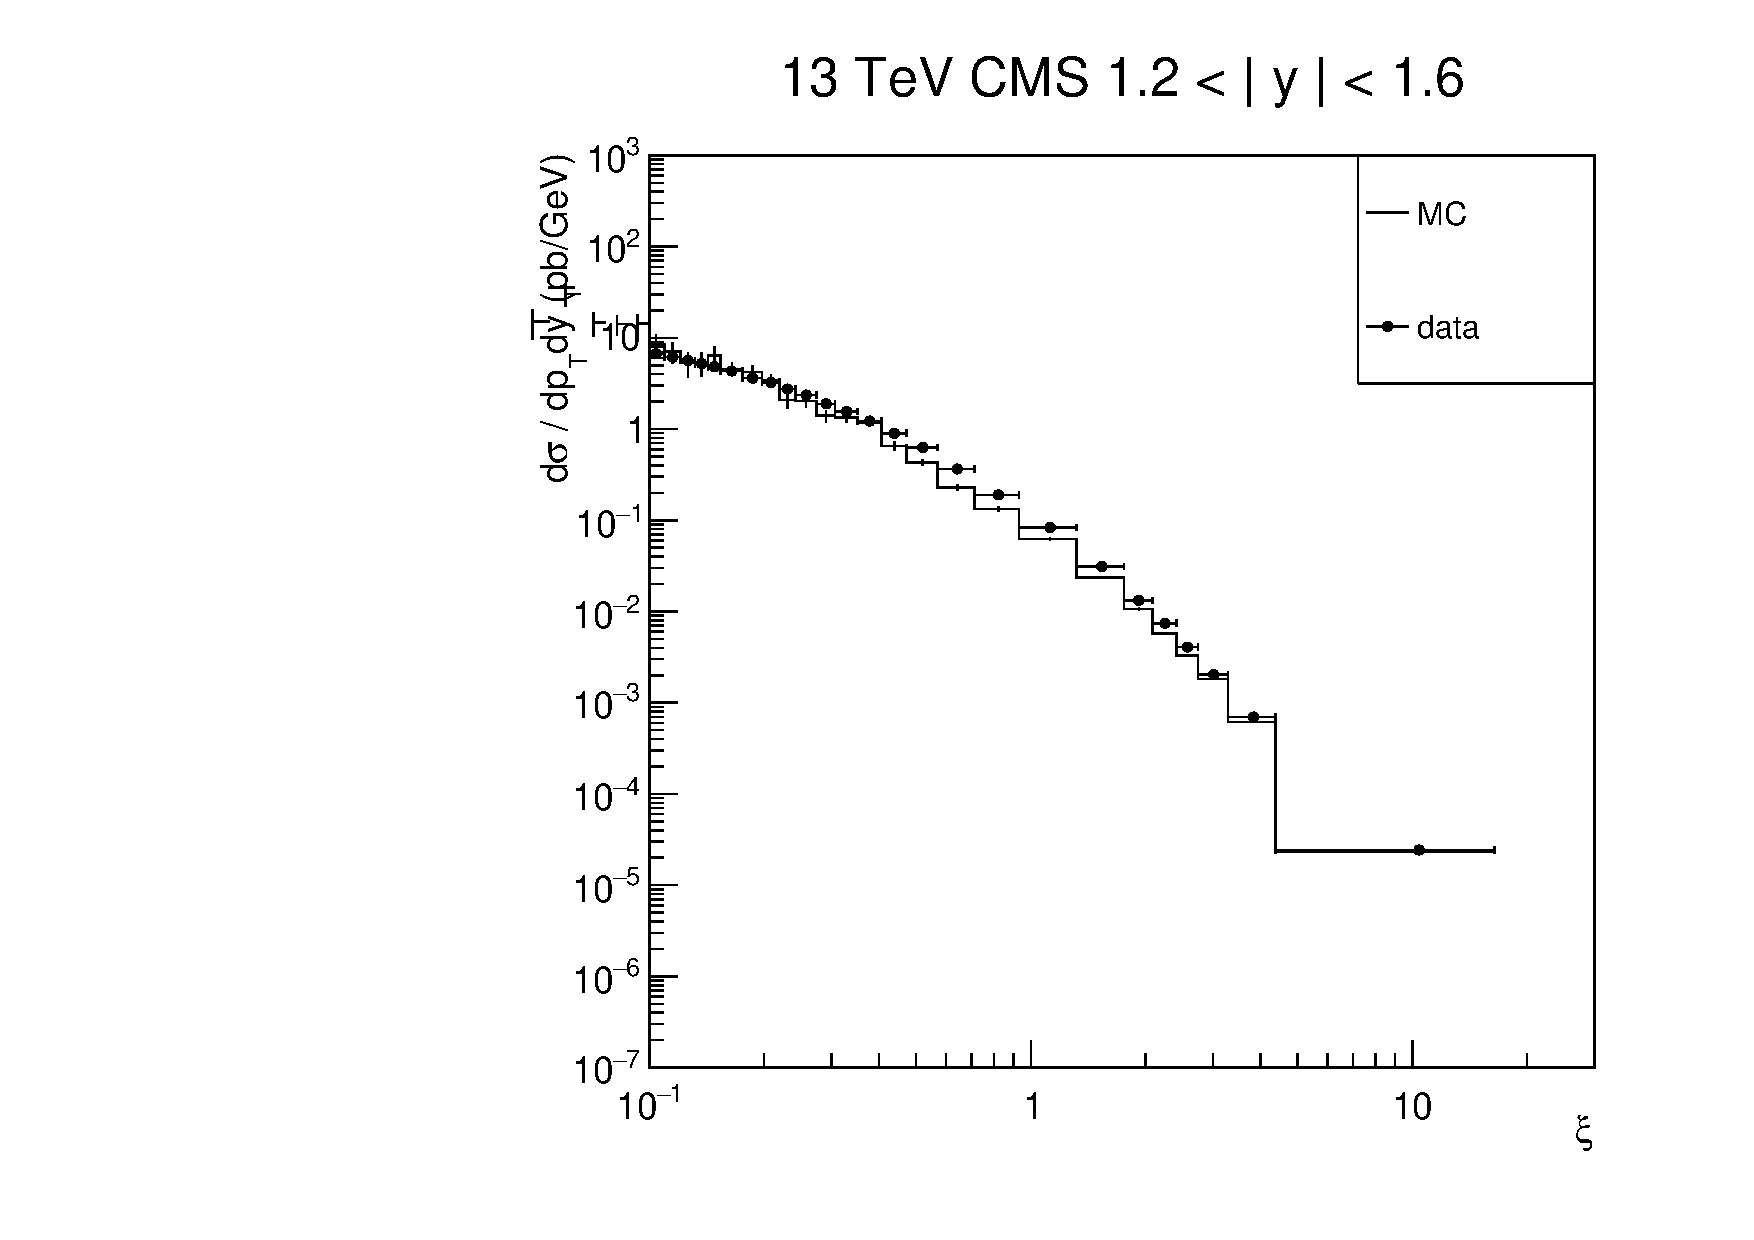
\includegraphics[width = 0.4\textwidth]{xi_13_C_y4.pdf}

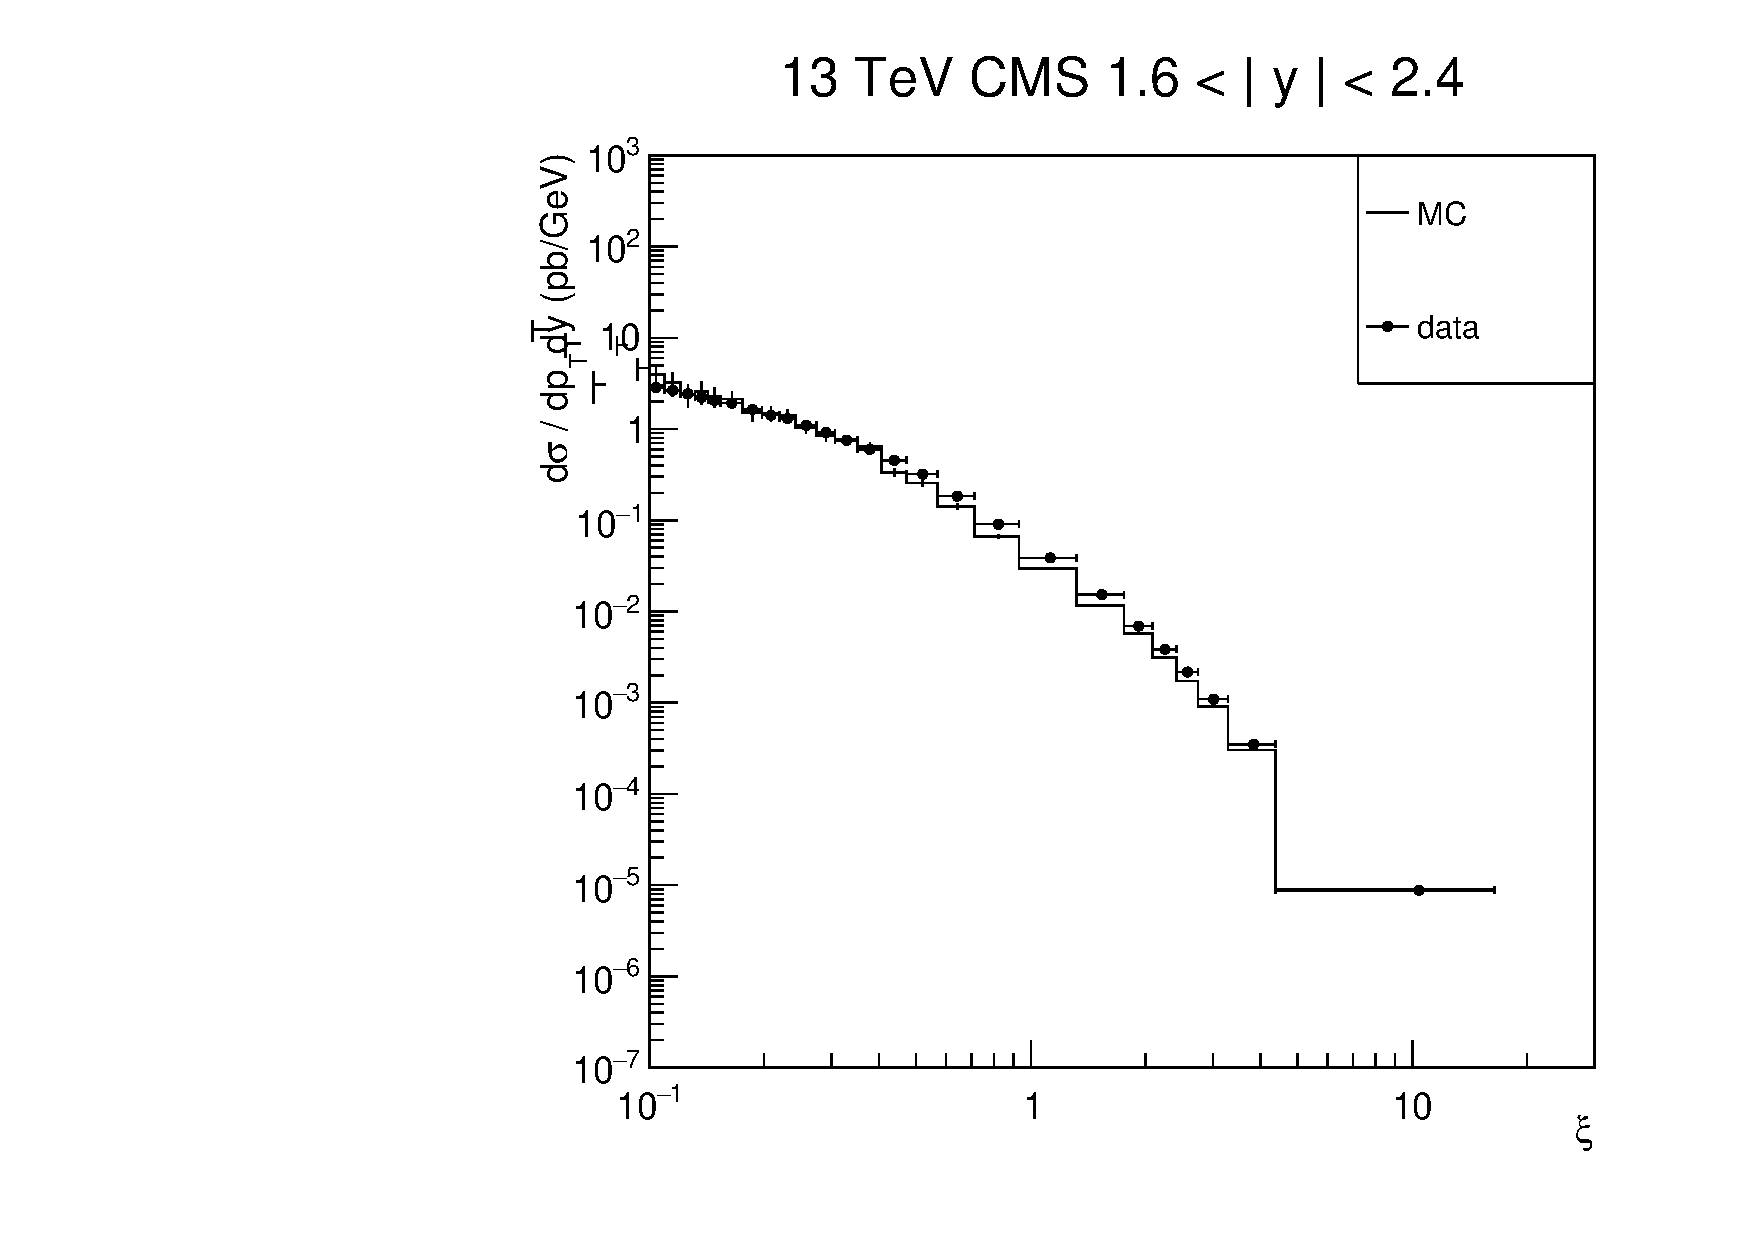
\includegraphics[width = 0.4\textwidth]{xi_13_C_y5.pdf}
%\caption{Comparison between MC $\xi$ distribution and data points in the six $y$ bins of the data, for 8 TeV. All histograms divided by total nr events and multiplied by same normalization factor. Data is not scaled.}\label{f:xi_comp}
\end{figure}

\end{document}